% THIS TEMPLATE IS A WORK IN PROGRESS
% Adapted from an original template by faculty at Reykjavik University, Iceland

\documentclass{scrartcl}

% Adapted from an original template by Hlyni Arnórssyni, Reykjavik University, Iceland
%
% ------------------------------ SETTINGS
\usepackage{geometry}

\geometry{
	paper=a4paper, % Paper size
	top=2.5cm, % Top margin
	bottom=2.5cm, % Bottom margin
	left=2.5cm, % Left margin
	right=2.4cm, % Right margin
	headheight=0.75cm, % Header height
	footskip=1.5cm, % Space from the bottom margin to the baseline of the footer
	headsep=0.75cm, % Space from the top margin to the baseline of the header
	%showframe, % Uncomment to show how the type block is set on the page
}

\usepackage{blindtext}
%-------------------------------- Character encoding ----------------------------
\usepackage[T1]{fontenc}
\usepackage[utf8]{inputenc}

%----------------------------- Mathematics packages from AMS ---------------

\usepackage{amsmath, amsfonts, amsthm, amssymb}
\usepackage{braket, nicefrac}

% ----------- International System of Units
\usepackage{siunitx}

%------------------------------ Lists / numbers -------------------------
\usepackage{enumitem, multicol}

%------------------------------- Figure insertions --------------
\usepackage{graphicx, float}  % Use option [H] to force the placement of a figure
\usepackage{keystroke}
\usepackage{pgfplots}\usepgfplotslibrary{units}\pgfplotsset{compat=1.16}




%%%%%%%%%%%%%%%%%%%%%%%%%% Hyperlink References %%%%%%%%%%%%%%%%%%%%%%%%%%%
\usepackage{hyperref}

%--------------------% Storage Path for images %-----------------%
\graphicspath{{graphics/}{Graphics/}{./}}
\usepackage{graphicx,epsfig}
\usepackage{graphicx}%
\usepackage{multirow}%
\usepackage{amsmath,amssymb,amsfonts}%
\usepackage{amsthm}%
\usepackage{mathrsfs}%
\usepackage[title]{appendix}%
\usepackage{xcolor}%
\usepackage{textcomp}%
\usepackage{manyfoot}%
\usepackage{booktabs}%
\usepackage{algorithm}%
\usepackage{algorithmicx}%
\usepackage{algpseudocode}%
\usepackage{listings}%
\usepackage{multicol} % Add this package
\usepackage{hhline}
\usepackage{colortbl}
\usepackage{caption}
\usepackage{longtable}
\hypersetup{
   colorlinks   = true,                               %Colours links instead of ugly boxes
   urlcolor     = blue,                               %Colour for external hyper links
   linkcolor    = blue,                               %Colour of internal links
   citecolor    = red,                                %Colour of citations
   setpagesize  = false,
   linktocpage  = true,
}
\graphicspath{ {fig/} }



\renewenvironment{abstract}{
    \centering
    \textbf{Abstract}
    \vspace{0.5cm}
    \par\itshape
    \begin{minipage}{1\linewidth}}{\end{minipage}
    \noindent\ignorespaces
}
% ------------------------------------------------------------------------------------------------------------------------

\begin{document}
%Title of the report, name of coworkers and dates (of experiment and of report).
\begin{titlepage}
	\centering
	
\includegraphics[width=0.6\textwidth]{GW_logo.eps}\par
	\vspace{1cm}
	%%%% COMMENT OUT irrelevant lines below: Data Science OR Computer Science OR none
	{\scshape\LARGE Data Science Program \par}
	\vspace{1cm}
	{\scshape\Large Capstone Report - Spring 2024\par}
	%{\large \today\par}
	\vspace{1cm}
	%%%% PROJECT TITLE
	{\huge\bfseries A Benchmark for Graph-Based Dynamic Recommendation Systems\par}
	\vspace{1cm}
	%%%% AUTHOR(S)
	{\Large\itshape Tyler Wallett\\}\par
	\vspace{1cm}
	supervised by\par
	%%%% SUPERVISOR(S)
	Amir Jafari

	\vfill
	\begin{abstract}
	    \quad The surge of Graph Neural Networks (GNNs) has catalyzed significant advancements in recommendation systems by enabling more effective modeling of user-item interactions within undirected bipartite graphs. However, the proliferation of GNN architectures, coupled with the absence of standardized benchmarking frameworks, presents challenges in systematically evaluating and comparing different dynamic recommendation models. In response, we propose a comprehensive benchmarking study of bipartite GNN operators for recommendation systems using the PyTorch Geometric library. Our contributions include the development of a flexible benchmarking framework encompassing data preprocessing, model training, and evaluation protocols, facilitating fair comparison across diverse dynamic recommendation scenarios. We rigorously assess the performance of various GNN models, ranging from traditional methods to state-of-the-art architectures, on the MovieLens100k dataset. Through insightful analysis of experimental results, we elucidate the strengths and weaknesses of different GNN operators and offer practical suggestions for model selection and configuration. Our work aims to foster transparency, reproducibility, and innovation in GNN-based dynamic recommendation systems, providing a valuable resource for researchers and practitioners in the field.
	\end{abstract}
	\vfill
% Bottom of the page
\end{titlepage}
\tableofcontents
\newpage
% ------------------------------------------------------------------------------------------------------------------------
\section{Introduction}\label{sec1}

\quad In the realm of recommendation systems, the efficacy of modern algorithms is often evaluated on their ability to understand complex user-item interactions within undirected bipartite graphs. These interactions, which represent the relationships between users and items, are pivotal for generating accurate recommendations in various domains such as e-commerce, social media, and content streaming platforms. With the advent of Graph Neural Networks (GNNs), there has been a surge of interest in leveraging their expressive power to model and predict user preferences more effectively.

However, the landscape of GNN-based recommendation models is vast, encompassing diverse architectures, training strategies, and evaluation metrics. Amidst this diversity, there is a pressing need for a standardized benchmarking framework that enables fair comparison and evaluation of different GNN operators tailored specifically for undirected bipartite recommendation graphs.

In response to this need, we present a comprehensive benchmarking study of bipartite GNN operators for dynamic recommendation systems. Leveraging the PyTorch Geometric library, we meticulously evaluate a spectrum of GNN models, ranging from traditional methods to state-of-the-art architectures.

Thus, our contributions are threefold: \\ 

1. \underline{Benchmarking Framework Development}: We propose a flexible and extensible benchmarking framework that facilitates the systematic evaluation of GNN-based recommendation models. This framework encompasses data preprocessing, model training, evaluation protocols, and result analysis, thereby providing a standardized basis for fair comparison. \\ 

2. \underline{Model Selection and Evaluation}: We rigorously assess the performance of various bipartite GNN operators, including GraphSAGE, Graph Attention Networks (GATs), and more, under different experimental settings. By conducting extensive experiments on MovieLens100k dataset, we elucidate the strengths and weaknesses of each model in capturing intricate user-item interactions. \\ 

3. \underline{Insightful Analysis and Recommendations}: Through thorough analysis of experimental results, we uncover key insights into the behavior and performance of different bipartite GNN operators in dynamic recommendation scenarios. Based on these insights, we offer practical suggestions for selecting and configuring GNN models tailored to specific application domains. \\ 

By providing a comprehensive benchmarking study along with an open-source implementation in PyTorch Geometric, we aim to foster transparency, reproducibility, and innovation in the development of GNN-based dynamic recommendation systems. We believe that our work will serve as a valuable resource for researchers and practitioners seeking to leverage the power of GNNs for building more effective recommendation engines.



% ------------------------------------------------------------------------------------------------------------------------
\section{Methodology}

\quad The purpose of this section is to delineate the structured approach utilized for benchmarking PyTorch Geometric's bipartite GNN operators for dynamic recommendation systems. To fulfill this purpose this section introduces graph theory concepts for edge-level prediction for dynamic recommendation systems, provides an overview of the PyTorch Geometric pipeline, describes each model, and accounts for the dataset and metrics utilized.

\subsection{Graph Theory}

\quad Graphs, denoted by $G(V, E)$, consist of two finite sets, $V$ and $E$. Each element of $V = \{v_{1}, v_{2}, \ldots, v_{n}\}$ is called a vertex (node) and represents the entities within the graph. Each element of $E = \{ \{v_{1}, v_{2}\}, \ldots, \{v_{1}, v_{n}\}\}$ is called an edge (link) and represents the relationships between each vertex within the graph. To fully grasp the graph used for dynamic edge-level prediction for recommendation systems, we first need to understand three types of graphs: \\ 

\textbf{• Undirected graphs:} Graphs that lack inherent edge directionality, signifying mutual or symmetrical relationships between vertices. \\ 

\textbf{• Bipartite graphs:} Graphs, denoted as $G(U, V, E)$, that partition vertices into two disjoint sets $U$ and $V$, ensuring non-adjacency within sets and edges connecting vertices from distinct vertex sets. \\

\textbf{• Heterogeneous graphs:} Graphs that contain either two or more types of vertex sets or two or more types of edge sets. \\ 

Hence, for dynamic edge-level prediction for recommendation systems, we adopt an undirected bipartite graph, represented as $G(U, I, E)$, where $U$ denotes users and $I$ denotes recommended items. From this graph, the goal is to predict edges between users and items over time.

\subsection{PyTorch Geometric}

\begin{figure*}
    \centering
    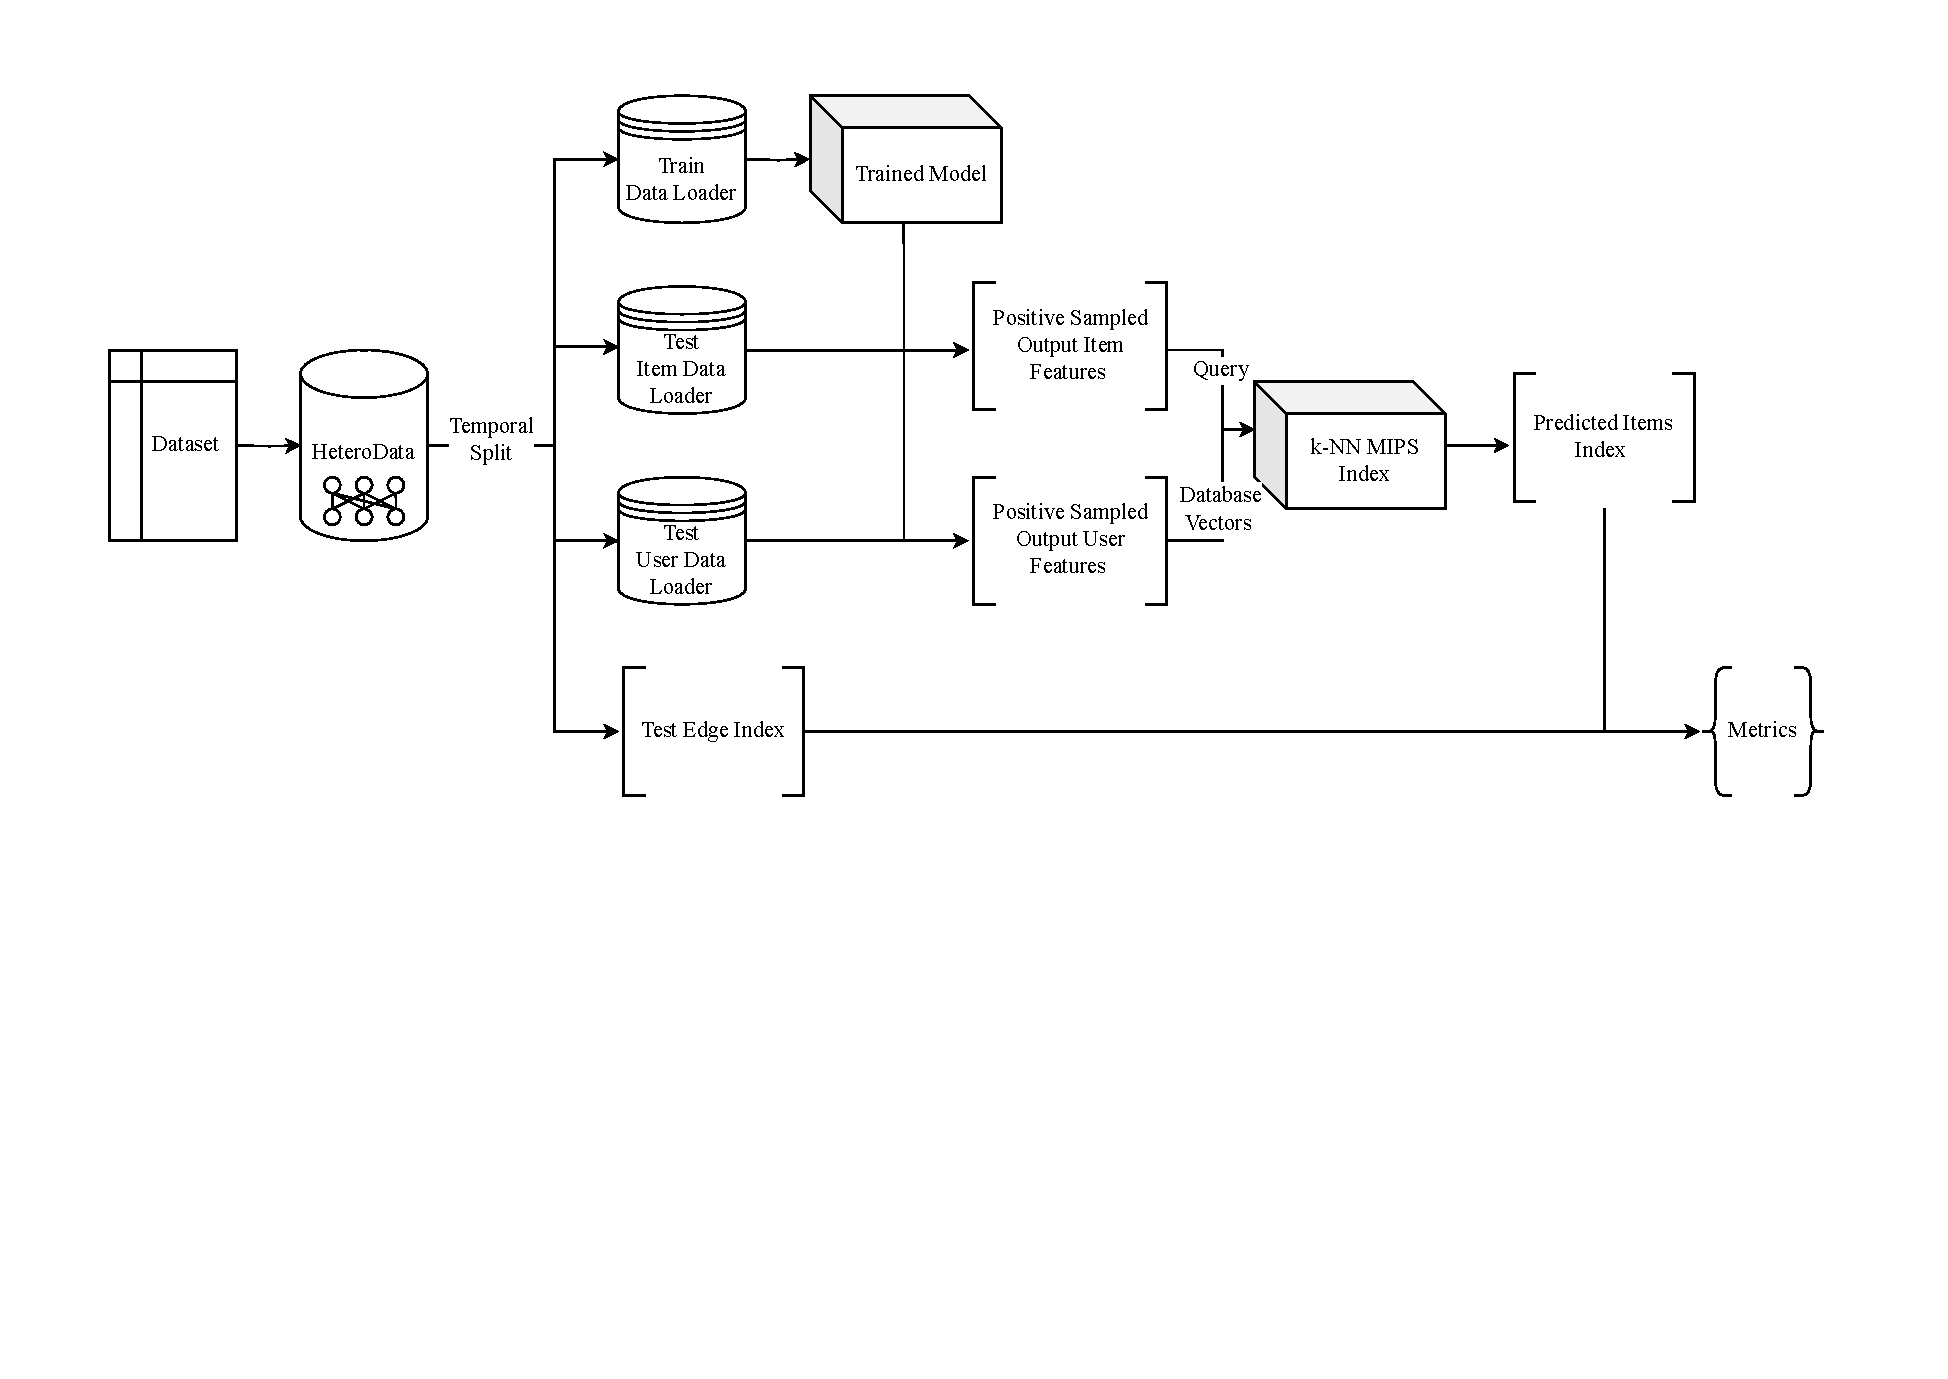
\includegraphics[width=\linewidth]{sn-article-template/imgs/PyTorchPipeline.drawio.pdf}
    \caption{PyTorch Geometric Dynamic Recommendation System Pipeline.}
    \label{fig:pytorch_geometric_pipeline}
\end{figure*}

\quad PyTorch Geometric is a powerful Python library used for developing GNNs that is seamlessly integrated with PyTorch. It offers intuitive functionalities for heterogeneous graph learning and data structures, data loaders, bipartite GNN operators, and $k$-Nearest Neighbors Maximum Inner Product Search ($k$-NN MIPS). PyTorch Geometric plays an indispensable role, as the entire benchmark project relies on its pipeline \ref{fig:pytorch_geometric_pipeline}. You can find the code used for this benchmark here: \href{https://github.com/twallett/DynamicRecSys}{https://github.com/twallett/DynamicRecSys}. 

Now, let's delve into a detailed explanation of each component comprising the PyTorch Geometric pipeline, outlining the structure of the evaluation process: \\

\textbf{• HeteroData:} HeteroData is a data structure in PyTorch Geometric that encompasses each component of a heterogeneous graph. Utilizing this data structure is the first step of the pipeline \ref{fig:pytorch_geometric_pipeline} as we are interested in representing our comma-separated values (csv) dataset as a heterogeneous graph. Specifically, for dynamic edge-level prediction for recommendation systems, we are interested in representing the previously mentioned undirected bipartite graph $G(U,I,E)$. 

The structure of $G(U,I,E)$ is characterized by three main components. Each user vertex inside the user vertex set $U$ is represented by an embedding vector, or vertex feature, $U=[\mathbf{x}_{user_{1}},\mathbf{x}_{user_{2}}, ..., \mathbf{x}_{user_{|U|}}]$. These user embeddings are first initialized with an identity matrix $I$ of dimension $|U|x|U|$. Similarly, each item vertex inside the item vertex set $I$ is represented by an embedding vector, or vertex feature, $I=[\mathbf{x}_{item_{1}},\mathbf{x}_{item_{2}}, ..., \mathbf{x}_{item_{|I|}}]$. However, the only difference is that these item embeddings are initialized with normal distributed random numbers in a matrix of size $|I|xLatent \ Dimension$, where the latent dimension is a hyperparameter. Lastly, edges are represented by a bidirectional edge index (adjacency matrix) with feature and time labels for user-feature-item and item-feature-user relationships. \\

\textbf{• Data Loaders:} In the pipeline \ref{fig:pytorch_geometric_pipeline}, before constructing the data loaders there is a temporal split of the dataset. To do so, we simply extract the HeteroData time labels and sort them to be split by a set threshold.

LinkNeighborhood Loader is the data loader used for training the models. This data loader samples bipartite edges from the graph $G(U,I,E)$ with temporal considerations. It specifies parameters such as the number of neighbors to be sampled, batch size, and temporal attributes in the graph data. Additionally, it sets up edge labels and their associated indices, while controlling the ratio of negative to positive edges to be sampled during training. 

Neighborhood Loader\cite{sageconv} is the data loader used for testing the models. This data loader samples unidirectional edges from the graph $G(U,I,E)$ with temporal considerations, and handles the same parameters as previously mentioned for the LinkNeighborhood Loader.

Note that, in the pipeline \ref{fig:pytorch_geometric_pipeline}, a test edge index is also created. This test edge index will be compared to the predicted item’s index to prepare the link-prediction metrics. \\ 

\textbf{• Heterogeneous Graph Learning:} Heterogeneous Graph Learning refers to any GNN learning on heterogeneous graph data. One of the challenges faced is that Standard Message Passing GNNs (MP-GNNs) can not trivially be applied to heterogeneous graph data, as vertex and edge features from different types can not be processed by the same functions due to differences in feature type. Luckily, PyTorch Geometric provides functionality to automatically convert a homogeneous GNN model to a heterogeneous GNN model. 

In the pipeline \ref{fig:pytorch_geometric_pipeline} the design of the trained model is standardized for all models. As the LinkNeighborhood Loader samples training edges in a bidirectional and temporal manner, it also samples corresponding input embeddings. For dynamic edge-level prediction for recommendation systems, these sampled input embeddings can be from either the user $\mathbf{x}_{user_{j}}$ or item $\mathbf{x}_{item_{j}}$. Once these input embeddings are sampled they are passed through a bipartite GNN model, or simply viewed as an $\textbf{encoder}$ function: \\ 

\begin{center}
    $\mathbf{x}^{\prime}_{item_{i}} = \textbf{encoder}(\mathbf{x}_{item_{j}})$ \\~\\ 
    $\mathbf{x}^{\prime}_{user_{i}} = \textbf{encoder}(\mathbf{x}_{user_{j}})$ \\~\\
\end{center} 

After receiving output embeddings for both user $\mathbf{x}^{\prime}_{user_{i}}$ and item $\mathbf{x}^{\prime}_{item_{i}}$, these are then passed through a $\textbf{decoder}$ function to return an output vector $\mathbf{a}$  (Note that the choice of $\textbf{decoder}$ function for this benchmark was simply an inner product between the two sampled output embeddings): \\ 

\begin{center}
    $\mathbf{a} = \textbf{decoder}(\mathbf{x}^{\prime}_{item_{i}},\mathbf{x}^{\prime}_{user_{i}})$ \\~\\
\end{center} 

Lastly, the output $\mathbf{a}$ of this $\textbf{decoder}$ function is used to calculate a mean squared error $e$ relative to the sampled edge labels $\mathbf{t}$:

\begin{center}
    $e = \frac{1}{n} \sum_{i=1}^{n} (\mathbf{t} - \mathbf{a})^2$\\~\\
\end{center}

By following this procedure, that applies heterogeneous graph learning functionality, we are able to standardize the training of all of the bipartite GNN models. \\ 

\textbf{• $k$-NN MIPS:} Maximum Inner Product Search (MIPS) is an algorithmic technique designed to efficiently find an optimal database vector $\mathbf{x_{*}}$ by maximizing the inner product similarity measure between a corresponding database vector $\mathbf{x}$ and query vector $\mathbf{q}$. There are many variations of MIPS, one of them being Nearest Neighbor MIPS\cite{nnmips1, nnmips2} attempting to find the optimal database vector $\mathbf{x_{*}}$ by minimizing over a distance function $\rho$: \\ 

\begin{center}
    $\mathbf{x_{*}} = argmin \ \rho(\mathbf{q}^T \mathbf{x})$\\~\\
\end{center}

$k$-Nearest Neighbor MIPS\cite{nnmips3} is simply an extension of Nearest Neighbor MIPS that attempts to find optimal spatial relationships within a neighborhood of $k$ expansions.
PyTorch Geometric provides $k$-Nearest Neighbor MIPS\cite{nnmips3} integration by means of the Faiss library\cite{faiss}. Therefore, we are able to calculate $k$ optimal spatial relationships between users and items at inference within our pipeline \ref{fig:pytorch_geometric_pipeline}. \\ 

\textbf{• Metrics:} In the evaluation of dynamic recommendation systems, various metrics play crucial roles in quantifying the effectiveness and performance of the models. These metrics provide insights into how well the system is able to suggest relevant items to users. 

Recall@$k$ and Precision@$k$ are fundamental measures that assess the accuracy and completeness of recommendations within the top-$k$ suggestions, respectively. 

\[
\text{Recall@}k = \frac{\text{Relevant items in top-} k\text{ recommendations}}{\text{Total number of relevant items}}
\]

\[
\text{Precision@}k = \frac{\text{Relevant items in top-} k\text{ recommendations}}{k}
\]

Mean Average Precision@$k$ (MAP@$k$) takes into account the precision of recommendations at different cutoff levels, providing a holistic view of the system's performance. 

\[
\text{MAP@}k = \frac{1}{|Q|} \sum_{q=1}^{|Q|} \frac{1}{\min(k, N_q)} \sum_{i=1}^k P(i)
\] \\ 

F1@$k$ offers a balanced evaluation by considering both precision and recall at the $k$-th recommendation. 

\[ F1@k = 2 \times \frac{\text{Precision@$k$} \times \text{Recall@$k$}}{\text{Precision@$k$} + \text{Recall@$k$}} \] \\ 

Normalized Discounted Cumulative Gain@$k$ (nDCG@$k$) evaluates the ranking quality of recommended items up to the $k$-th recommendation, considering both relevance and position in the list. 

\[ \text{DCG@$k$} = \sum_{i=1}^{k} \frac{2^{rel_i} - 1}{\log_2(i+1)} \]
\[ \text{IDCG@$k$} = \sum_{i=1}^{\text{min}(k, \text{num\_relevant})} \frac{2^{rel_i} - 1}{\log_2(i+1)} \]
\[ \text{nDCG@$k$} = \frac{\text{DCG@$k$}}{\text{IDCG@$k$}} \] \\ 

Together, these metrics offer a comprehensive assessment of dynamic recommendation systems, crucial for optimizing their performance and enhancing user satisfaction.

It is important to mention that the early stopping callback was configured with a patience parameter of 20, ensuring that training ceased when there was no improvement in performance over 20 consecutive epochs. The validation score was conducted based on Recall@$k$ since we prioritize the identification of all relevant items, thus emphasizing the system's ability to minimize the likelihood of overlooking potentially suitable recommendations. This choice aligns with the practical objectives of our research, which emphasize the importance of providing high-quality recommendations to users.

\subsection{Models}

\quad In total 13 bipartite GNN operators from Pytorch Geometric were trained. Each model was trained for 1000 epochs using a batch size of 1024 and Stochastic Gradient Descent (SGD) optimization with a learning rate of 3e-03. Further, each model operates with a latent dimension of 64 and samples neighbors with a proximity of [2,2] for a equivalent benchmarking. For specific information regarding the hyperparameters used for the training of each of these models refer to the summary table in the appendix section \ref{tab:hyperparameters}.

Several bipartite GNN models were not included in the benchmarking. Models that necessitated edge labels, our targets $\mathbf{t}$, to be passed as inputs were obviously excluded, these are: GINEConv\cite{gineconv}, GMMConv\cite{gmmconv}, SplineConv\cite{splineconv}, NNConv\cite{nnconv}, CGConv\cite{cgconv}, and GeneralConv\cite{generalconv}. Lastly, models that required building a different pipeline were also excluded, such as MFConv\cite{mfconv} and FAConv\cite{faconv}.

Additionally, for each bipartite GNN operator, random seeds were set and temporal sampling was run on central processing units (CPUs), thus ensuring the reproducibility of results.


\subsubsection{SimpleConv}

\quad The SimpleConv (Simple Convolutional Layer) model operates by aggregating information from neighboring items or users. It adopts a simple aggregation strategy where the embedding vector of an item or user is updated by aggregating the embeddings of its neighboring items or users using an aggregation operator. In mathematical terms, for each item or user, denoted as $i$, its updated embedding, $\mathbf{x}^{\prime}_{item_i}$ or $\mathbf{x}^{\prime}_{user_i}$, is obtained by aggregating the embeddings of its neighbors, denoted as $j \in \mathcal{N}(i)$, where $\mathcal{N}(i)$ represents the set of neighbors of $i$, and $\bigoplus$ denotes the SetTransformerAggregation\cite{simpleconv} operation. This aggregation operator was chosen for this benchmark as it yielded the best results out of all of the aggregation operators. \\ 

\begin{center}
    $\mathbf{x}^{\prime}_{item_{i}} = \bigoplus_{j \in \mathcal{N}(i)} \mathbf{x}_{item_{j}}$ \\~\\
    $\mathbf{x}^{\prime}_{user_{i}} = \bigoplus_{j \in \mathcal{N}(i)} \mathbf{x}_{user_{j}}$
\end{center}

\subsubsection{SAGEConv\cite{sageconv}} 

\quad SAGEConv (GraphSAGE Convolutional Layer) updates the embeddings of items or users by incorporating information from both the target entity and its neighbors. Unlike SimpleConv, SAGEConv employs learnable weight matrices to compute the updates, enabling more flexibility and expressiveness in the model. Specifically, for each item or user, denoted as $i$, its updated embedding, $\mathbf{x}^{\prime}_{item_i}$ or $\mathbf{x}^{\prime}_{user_i}$, is calculated as a linear combination of its own embedding and a weighted average of its neighbors' embeddings. The weights for this combination are determined by the weight matrices $\mathbf{W}_1$ and $\mathbf{W}_2$. The first weight matrix $\mathbf{W}_1$ operates directly on the target entity's embedding, while the second weight matrix $\mathbf{W}_2$ operates on the mean of its neighbors' embeddings. \\ 

\begin{center}
    $\mathbf{x}^{\prime}_{item_{i}} = \mathbf{W}_1 \mathbf{x}_{item_{i}} + \mathbf{W}_2 \cdot \mathrm{mean}_{j \in \mathcal{N}(i)} \mathbf{x}_{item_{j}}$ \\~\\
    $\mathbf{x}^{\prime}_{user_{i}} = \mathbf{W}_1 \mathbf{x}_{user_{i}} + \mathbf{W}_2 \cdot \mathrm{mean}_{j \in \mathcal{N}(i)} \mathbf{x}_{user_{j}}$
\end{center}

\subsubsection{GraphConv\cite{graphconv}} 

\quad Similarly to SAGEConv, GraphConv (Graph Convolutional Layer) iteratively refines the embeddings of items or users by assimilating insights from both the focal entity and its surrounding neighbors within the graph. Additionally, GraphConv also integrates learnable weight matrices, $\mathbf{W}_1$ and $\mathbf{W}_2$, into its computation. However, unlike SAGEConv each item or user represented by $i$, its updated embedding, $\mathbf{x}^{\prime}_{item_i}$ or $\mathbf{x}^{\prime}_{user_i}$, is derived as a weighted sum of its own embedding and the aggregate of its neighbors' embeddings, instead of a weighted average. \\ 

\begin{center}
    $\mathbf{x}^{\prime}_{item_{i}} = \mathbf{W}_1 \mathbf{x}_{item_{i}} + \mathbf{W}_2 \cdot \sum_{j \in \mathcal{N}(i)} \mathbf{x}_{item_{j}}$ \\~\\
    $\mathbf{x}^{\prime}_{user_{i}} = \mathbf{W}_1 \mathbf{x}_{user_{i}} + \mathbf{W}_2 \cdot \sum_{j \in \mathcal{N}(i)} \mathbf{x}_{user_{j}}$
\end{center}

\subsubsection{ResGatedGraphConv\cite{resgatedgraphconv}} 

\quad ResGatedGraphConv (Residual Gated Graph Convolutional Layer) extends the conventional graph convolution by incorporating residual connections and gating mechanisms. The updated embeddings of items or users, denoted as $\mathbf{x}^{\prime}_{item_i}$ or $\mathbf{x}^{\prime}_{user_i}$, are computed through a combination of the original embeddings and the aggregated information from their neighboring entities within the graph. Specifically, for each item or user represented by $i$, the updated embedding is calculated as a weighted sum of its original embedding and the transformed embeddings of its neighbors, where the weighting factor $\eta_{i,j}$ is determined by a gating mechanism. This gating mechanism, governed by the sigmoid function $\sigma$, modulates the importance of neighboring embeddings based on their compatibility with the target entity's embedding, as encoded by the weight matrices $\mathbf{W}_3$ and $\mathbf{W}_4$. \\ 

\begin{center}
    $\mathbf{x}^{\prime}_{item_{i}} = \mathbf{W}_1 \mathbf{x}_{item_{i}} + \sum_{j \in \mathcal{N}(i)} \eta_{i,j} \odot \mathbf{W}_2 \mathbf{x}_{item_{j}}$\\ 
    $\eta_{i,j} = \sigma(\mathbf{W}_3 \mathbf{x}_{item_{i}} + \mathbf{W}_4
    \mathbf{x}_{item_{j}})$ \\~\\
    $\mathbf{x}^{\prime}_{user_{i}} = \mathbf{W}_1 \mathbf{x}_{user_{i}} + \sum_{j \in \mathcal{N}(i)} \eta_{i,j} \odot \mathbf{W}_2 \mathbf{x}_{user_{j}}$\\ 
    $\eta_{i,j} = \sigma(\mathbf{W}_3 \mathbf{x}_{user_{i}} + \mathbf{W}_4
    \mathbf{x}_{user_{j}})$
\end{center}


\subsubsection{GATConv\cite{gatconv}} 

\quad GATConv (Graph Attention Network Convolutional Layer) is designed to capture complex dependencies and attention mechanisms within the graph. The updated embeddings of items or users, denoted as $\mathbf{x}^{\prime}_{item_i}$ or $\mathbf{x}^{\prime}_{user_i}$ respectively, are computed using attention mechanisms to dynamically weight the contributions of neighboring embeddings. Specifically, for each item or user represented by $i$, the updated embedding is a linear combination of the original embedding and the weighted sum of the embeddings of its neighbors. The attention coefficients $\alpha_{i,j}$ are computed using a shared self-attention mechanism across all neighbors, where the attention weights are determined by the attention mechanism applied to the pair of embeddings $\mathbf{x}_{item_i}$ and $\mathbf{x}_{item_j}$ (or $\mathbf{x}_{user_i}$ and $\mathbf{x}_{user_j}$). The attention mechanism employs a LeakyReLU activation with a negative slope of 0.2 on a linear combination of the embeddings followed by a softmax function to ensure that the attention coefficients sum to one.\\ 

\begin{center}
    $\mathbf{x}^{\prime}_{item_{i}} = \alpha_{i,i}\mathbf{W}_{1}\mathbf{x}_{item_{i}} + \sum_{j \in \mathcal{N}(i)} \alpha_{i,j}\mathbf{W}_{2}\mathbf{x}_{item_{j}}$\\
    $\alpha_{i,j} =
    \frac{
    \exp\left(\mathrm{LeakyReLU}\left(
    \mathbf{a}^{\top}_{1} \mathbf{W}_{1}\mathbf{x}_{item_{i}}
    + \mathbf{a}^{\top}_{2} \mathbf{W}_{2}\mathbf{x}_{item_{j}}
    \right)\right)}
    {\sum_{k \in \mathcal{N}(i) \cup \{ i \}}
    \exp\left(\mathrm{LeakyReLU}\left(
    \mathbf{a}^{\top}_{1} \mathbf{W}_{1}\mathbf{x}_{item_{i}}
    + \mathbf{a}^{\top}_{2}\mathbf{W}_{2}\mathbf{x}_{item_{k}}
    \right)\right)}$ \\~\\
    $\mathbf{x}^{\prime}_{user_{i}} = \alpha_{i,i}\mathbf{W}_{1}\mathbf{x}_{user_{i}} + \sum_{j \in \mathcal{N}(i)} \alpha_{i,j}\mathbf{W}_{2}\mathbf{x}_{user_{j}}$\\
    $\alpha_{i,j} =
    \frac{
    \exp\left(\mathrm{LeakyReLU}\left(
    \mathbf{a}^{\top}_{1} \mathbf{W}_{1}\mathbf{x}_{user_{i}}
    + \mathbf{a}^{\top}_{2} \mathbf{W}_{2}\mathbf{x}_{user_{j}}
    \right)\right)}
    {\sum_{k \in \mathcal{N}(i) \cup \{ i \}}
    \exp\left(\mathrm{LeakyReLU}\left(
    \mathbf{a}^{\top}_{1} \mathbf{W}_{1}\mathbf{x}_{user_{i}}
    + \mathbf{a}^{\top}_{2}\mathbf{W}_{2}\mathbf{x}_{user_{k}}
    \right)\right)}$
\end{center}

\subsubsection{GATv2Conv\cite{gatv2conv}} 

\quad GATv2Conv (Graph Attention Network v2 Convolutional Layer) is an improvement of GATConv aimed at solving static attention coefficients. Similarly, GATv2Conv employs attention mechanisms to dynamically weigh the contributions of neighboring embeddings in a graph. The updated embeddings of items or users, denoted as $\mathbf{x}^{\prime}_{item_i}$ or $\mathbf{x}^{\prime}_{user_i}$ respectively, are computed using attention coefficients $\alpha_{i,j}$ determined by an self-attention mechanism. These attention coefficients control the influence of neighboring embeddings in the computation of updated embeddings. However, GATv2Conv solves the problem of static attention coefficients by applying attention mechanism directly on the concatenation of node embeddings before applying the LeakyReLU activation function. \\

\begin{center}
    $\mathbf{x}^{\prime}_{item_{i}} = \alpha_{i,i}\mathbf{W}_{1}\mathbf{x}_{item_{i}} + \sum_{j \in \mathcal{N}(i)} \alpha_{i,j}\mathbf{W}_{2}\mathbf{x}_{item_{j}}$ \\ 
    $\alpha_{i,j} = \frac{\exp\left(\mathbf{a}^{\top}\mathrm{LeakyReLU}\left(\mathbf{W}_{1} \mathbf{x}_{item_{i}} + \mathbf{W}_{2} \mathbf{x}_{item_{j}}\right)\right)}{\sum_{k \in \mathcal{N}(i) \cup \{ i \}} \exp\left(\mathbf{a}^{\top}\mathrm{LeakyReLU}\left(\mathbf{W}_{1} \mathbf{x}_{item_{i}} + \mathbf{W}_{2} \mathbf{x}_{item_{k}}\right)\right)}$ \\~\\
    $\mathbf{x}^{\prime}_{user_{i}} = \alpha_{i,i}\mathbf{W}_{1}\mathbf{x}_{user_{i}} + \sum_{j \in \mathcal{N}(i)} \alpha_{i,j}\mathbf{W}_{2}\mathbf{x}_{user_{j}}$ \\ 
    $\alpha_{i,j} = \frac{\exp\left(\mathbf{a}^{\top}\mathrm{LeakyReLU}\left(\mathbf{W}_{1} \mathbf{x}_{user_{i}} + \mathbf{W}_{2} \mathbf{x}_{user_{j}}\right)\right)}{\sum_{k \in \mathcal{N}(i) \cup \{ i \}} \exp\left(\mathbf{a}^{\top}\mathrm{LeakyReLU}\left(\mathbf{W}_{1} \mathbf{x}_{user_{i}} + \mathbf{W}_{2} \mathbf{x}_{user_{k}}\right)\right)}$
\end{center}

\subsubsection{TransformerConv\cite{transformerconv}} 

\quad TransformerConv (Transformer Convolutional Layer) introduces a novel convolutional operation inspired by the Transformer\cite{transformer} architecture. The updated embeddings of items or users, denoted as $\mathbf{x}^{\prime}_{item_i}$ or $\mathbf{x}^{\prime}_{user_i}$, are computed as a weighted sum of the original embeddings of neighboring entities, where the attention weights $\alpha_{i,j}$ are determined through a self-attention mechanism. This mechanism computes the attention scores between the embeddings of the target entity and its neighbors using trainable weight matrices $\mathbf{W}_3$ and $\mathbf{W}_4$, followed by a softmax operation to ensure a valid probability distribution. Additionally, a scaling factor $\sqrt{d}$ is applied to stabilize the gradients during training, where $d$ represents the dimensionality of the embeddings. \\ 

\begin{center}
    $\mathbf{x}^{\prime}_{item_{i}} = \mathbf{W}_1 \mathbf{x}_{item_{i}} + \sum_{j \in \mathcal{N}(i)} \alpha_{i,j} \mathbf{W}_2 \mathbf{x}_{item_{j}}$ \\
    $\alpha_{i,j} = \textrm{softmax} \left( \frac{(\mathbf{W}_3\mathbf{x}_{item_{i}})^{\top} (\mathbf{W}_4\mathbf{x}_{item_{j}})} {\sqrt{d}} \right)$ \\~\\
    $\mathbf{x}^{\prime}_{user_{i}} = \mathbf{W}_1 \mathbf{x}_{user_{i}} + \sum_{j \in \mathcal{N}(i)} \alpha_{i,j} \mathbf{W}_2 \mathbf{x}_{user_{j}}$ \\
    $\alpha_{i,j} = \textrm{softmax} \left( \frac{(\mathbf{W}_3\mathbf{x}_{user_{i}})^{\top} (\mathbf{W}_4\mathbf{x}_{user_{j}})} {\sqrt{d}} \right)$ 
\end{center}

\subsubsection{GINConv\cite{ginconv}} 

\quad GINConv (Graph Isomorphism Network Convolutional Layer) introduces a convolutional operation that leverages neural networks. The updated embeddings of items or users, denoted as $\mathbf{x}^{\prime}_{item_i}$ or $\mathbf{x}^{\prime}_{user_i}$ respectively, are computed using a neural network $NN_{\mathbf{\Theta}}$ with learnable parameters $\mathbf{\Theta}$. The operation involves a combination of the original embeddings of the target entity and its neighbors, scaled by a factor $(1 + \epsilon)$, where $\epsilon$ is a small constant. \\ 

\begin{center}
    $\mathbf{x}^{\prime}_{item_{i}} = NN_{\mathbf{\Theta}} \left( (1 + \epsilon) \cdot \mathbf{x}_{item_{i}} + \sum_{j \in \mathcal{N}(i)} \mathbf{x}_{item_{j}} \right)$ \\~\\
    $\mathbf{x}^{\prime}_{user_{i}} = NN_{\mathbf{\Theta}} \left( (1 + \epsilon) \cdot \mathbf{x}_{user_{i}} + \sum_{j \in \mathcal{N}(i)} \mathbf{x}_{user_{j}} \right)$
\end{center}

\subsubsection{EdgeConv\cite{edgeconv}} 

\quad Similarly to GINConv, EdgeConv (Edge Convolutional Layer) introduces a convolutional operation that leverages neural networks. The updated embeddings of items or users, denoted as $\mathbf{x}^{\prime}_{item_i}$ or $\mathbf{x}^{\prime}_{user_i}$ respectively, are computed by aggregating information from neighboring entities within the graph. For each item or user represented by $i$, the updated embedding is obtained by summing over the embeddings of its neighbors, where each neighbor's embedding is transformed through a neural network $NN_{\mathbf{\Theta}}$ with learnable parameters $\mathbf{\Theta}$. However, unlike GINConv the transformation involves concatenating the original embedding of the target entity with the difference between the neighbor's embedding and the target entity's embedding. \\ 

\begin{center}
    $\mathbf{x}^{\prime}_{item_{i}} = \sum_{j \in \mathcal{N}(i)} NN_{\mathbf{\Theta}}(\mathbf{x}_{item_{i}} \, \Vert \, \mathbf{x}_{item_{j}} - \mathbf{x}_{item_{i}})$ \\~\\
    $\mathbf{x}^{\prime}_{user_{i}} = \sum_{j \in \mathcal{N}(i)} NN_{\mathbf{\Theta}}(\mathbf{x}_{user_{i}} \, \Vert \, \mathbf{x}_{user_{j}} - \mathbf{x}_{user_{i}})$
\end{center}


\subsubsection{FeaStConv\cite{feastconv}} 

\quad FeaStConv (Feature-Steered Convolutional Layer) is another  convolutional operation that attempts to employ an attention mechanism. The updated embeddings of items or users, denoted as $\mathbf{x}^{\prime}_{item_i}$ or $\mathbf{x}^{\prime}_{user_i}$ respectively, are computed by aggregating information from neighboring entities within the graph. Specifically, for each item or user represented by $i$, the updated embedding is obtained by averaging over the embeddings of its neighbors, weighted by a feature-steering mechanism $q_h(\mathbf{x}_{item_i}, \mathbf{x}_{item_j})$ or $q_h(\mathbf{x}_{user_i}, \mathbf{x}_{user_j})$ for items or users, respectively, where $h$ denotes an attention head. This mechanism, parameterized by learnable vectors $\mathbf{u}_h$ and biases $c_h$, steers the convolutional process towards relevant features by computing attention scores based on the feature differences between the target entity and its neighbors. The weighted sum is then multiplied by learnable weight matrices $\mathbf{W}_h$ to produce the final updated embedding. \\ 

\begin{center}
    $\mathbf{x}^{\prime}_{item_{i}} = \frac{1}{|\mathcal{N}(i)|} \sum_{j \in \mathcal{N}(i)} \sum_{h=1}^H
    q_h(\mathbf{x}_{item_{i}}, \mathbf{x}_{item_{j}}) \mathbf{W}_h \mathbf{x}_{item_{j}}$ \\
    $q_h(\mathbf{x}_{item_{i}}, \mathbf{x}_{item_{j}}) = \mathrm{softmax}_{j}
    (\mathbf{u}_h^{\top} (\mathbf{x}_{item_{j}} - \mathbf{x}_{item_{i}}) + c_h)$
    \\~\\
    $\mathbf{x}^{\prime}_{user_{i}} = \frac{1}{|\mathcal{N}(i)|} \sum_{j \in \mathcal{N}(i)} \sum_{h=1}^H
    q_h(\mathbf{x}_{user_{i}}, \mathbf{x}_{user_{j}}) \mathbf{W}_h \mathbf{x}_{user_{j}}$ \\ 
     $q_h(\mathbf{x}_{user_{i}}, \mathbf{x}_{user_{j}}) = \mathrm{softmax}_j
    (\mathbf{u}_h^{\top} (\mathbf{x}_{user_{j}} - \mathbf{x}_{user_{i}}) + c_h)$
\end{center}


\subsubsection{LEConv\cite{leconv}} 

\quad LEConv (Linear Embedding Convolutional Layer) is a convolutional operation that focuses on capturing linear relationships between entities within the graph. The updated embeddings of items or users, denoted as $\mathbf{x}^{\prime}_{item_i}$ or $\mathbf{x}^{\prime}_{user_i}$ respectively, are computed by combining the original embeddings with the differences between the transformed embeddings of the target entity and its neighbors. For each item or user represented by $i$, the updated embedding is obtained by multiplying the original embedding with $\mathbf{W}_1$ and summing over the differences between the transformed embeddings of the target entity and its neighbors, weighted by $\mathbf{W}_2$ and $\mathbf{W}_3$. \\ 

\begin{center}
    $\mathbf{x}^{\prime}_{item_{i}} = \mathbf{W}_1 \mathbf{x}_{item_{i}} +
    \sum_{j \in \mathcal{N}(i)}
    (\mathbf{W}_2 \mathbf{x}_{item_{i}} - \mathbf{W}_3 \mathbf{x}_{item_{j}})$ \\~\\
    $\mathbf{x}^{\prime}_{user_{i}} = \mathbf{W}_1 \mathbf{x}_{user_{i}} +
    \sum_{j \in \mathcal{N}(i)}
    (\mathbf{W}_2 \mathbf{x}_{user_{i}} - \mathbf{W}_3 \mathbf{x}_{user_{j}})$
\end{center}

\subsubsection{GENConv\cite{genconv}} 

\quad GENConv (Graph Edge Network Convolutional Layer) is a convolutional operation that leverages multi-layered perceptrons (MLPs). The updated embeddings of items or users, denoted as $\mathbf{x}^{\prime}_{item_i}$ or $\mathbf{x}^{\prime}_{user_i}$ respectively, are computed by applying a MLP to the sum of the original embedding of the target entity and the ReLU-activated sum of the embeddings of its neighbors, where $\epsilon$ is a small constant for numerical stability. \\ 

\begin{center}
    $\mathbf{x}_{item_{i}}^{\prime} = \mathrm{MLP} \left( \mathbf{x}_{item_{i}} +
    \sum_{j \in \mathcal{N}(i)} 
    \mathrm{ReLU} \left( \mathbf{x}_{item_{j}} \right) +\epsilon \right)$ \\~\\
    $\mathbf{x}_{user_{i}}^{\prime} = \mathrm{MLP} \left( \mathbf{x}_{user_{i}} +
    \sum_{j \in \mathcal{N}(i)} 
    \mathrm{ReLU} \left( \mathbf{x}_{user_{j}} \right) +\epsilon \right)$ 
\end{center}

\subsubsection{WLConvContinuous\cite{wlconvcontinuous}} 

\quad WLConvContinuous (Weisfeiler-Lehman Convolutional Layer with Continuous Weights) is a convolutional operation that incorporates Weisfeiler-Lehman graph isomorphism test and continuous weighting mechanisms. The updated embeddings of items or users, denoted as $\mathbf{x}^{\prime}_{item_i}$ or $\mathbf{x}^{\prime}_{user_i}$ respectively, are computed by averaging the original embeddings of the target entity and its neighbors, weighted by the inverse of their degrees. Specifically, for each item or user represented by $i$, the updated embedding is obtained by taking half of the original embedding and half of the average of the embeddings of its neighbors, weighted by $\frac{1}{\text{deg}(i)}$. This weighting scheme ensures that entities with higher degrees contribute proportionally less to the final embedding, mitigating the influence of highly connected nodes in the graph. \\ 

\begin{center}
    $\mathbf{x}^{\prime}_{item_{i}} = \frac{1}{2}\big(\mathbf{x}_{item_{i}} +
    \frac{1}{\textrm{deg}(i)}
    \sum_{j \in \mathcal{N}(i)}  \mathbf{x}_{item_{j}} \big)$ \\~\\
    $\mathbf{x}^{\prime}_{user_{i}} = \frac{1}{2}\big(\mathbf{x}_{user_{i}} +
    \frac{1}{\textrm{deg}(i)}
    \sum_{j \in \mathcal{N}(i)} \mathbf{x}_{user_{j}} \big)$
\end{center}

\subsection{Dataset}

\quad The MovieLens100k dataset is a classic benchmark dataset widely used in recommendation system research. It consists of 100,000 timestamped ratings (from 1 to 5) given by users to approximately 1,000 movies. The dataset is composed of 4 main features, these are: user id's, movie id's, ratings and timestamps. Therefore, the corresponding rating, given by each user to a particular movie, will serve as our edge label, or target $\mathbf{t}$, which we will try to approximate using the previously mentioned bipartite GNN operators. 

For the purposes of this benchmark, we preprocessed ratings to include only those equal to or greater than 4, ensuring a focus on high-quality user preferences and emphasizing positive interactions with movies. A description of the resulting dataset after being preprocessed can be seen in table \ref{tab:dataset}. \\ 

\begin{center}
\begin{tabular}{|l|*{4}{c|}}
\hline
                        Dataset & Users    & Items    & Interactions   \\ \hline
MovieLens100k\cite{movielens}               & 942 & 1447 & 55,375 \\ \hline
\end{tabular}
\captionof{table}{Preprocessed MovieLens100k Description.}
\label{tab:dataset}
\end{center}

% ------------------------------------------------------------------------------------------------------------------------

\section{Results}

\begin{figure*}
\begin{center}
\begin{minipage}[b]{0.48\textwidth}
    \centering
    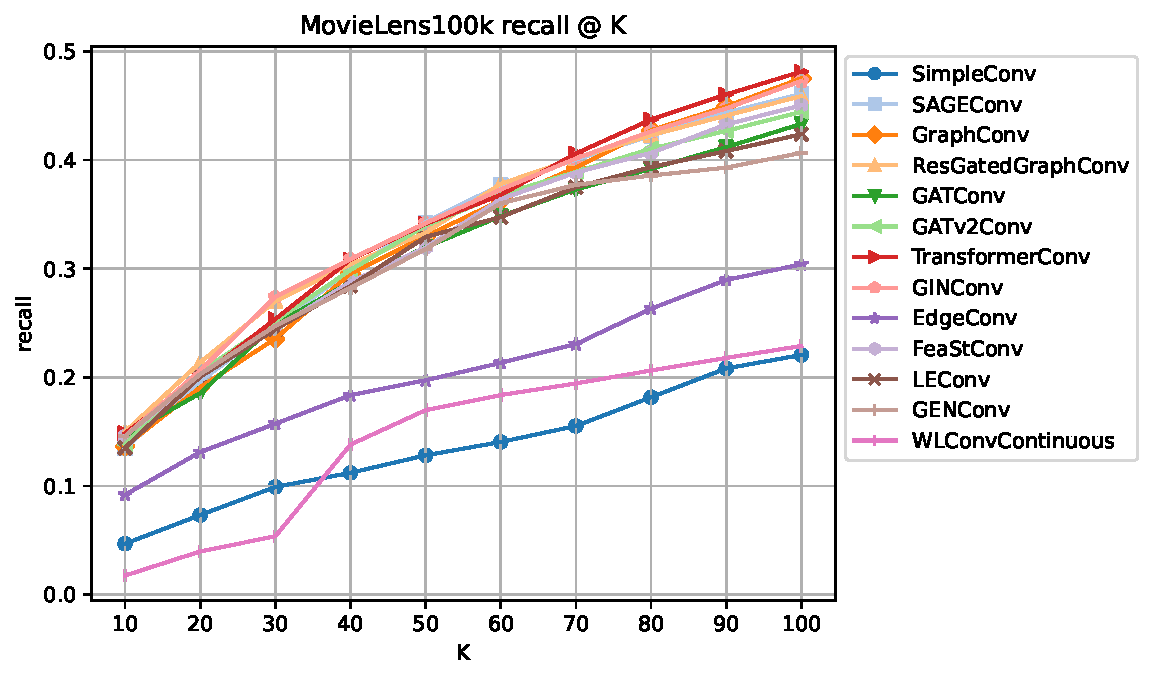
\includegraphics[width=\textwidth]{sn-article-template/imgs/MovieLens100k_recall.pdf}
    \captionof{figure}{MovieLens100k Results for Recall@$k$.}
    \label{fig:recall}
\end{minipage}
\hfill
\begin{minipage}[b]{0.48\textwidth}
    \centering
    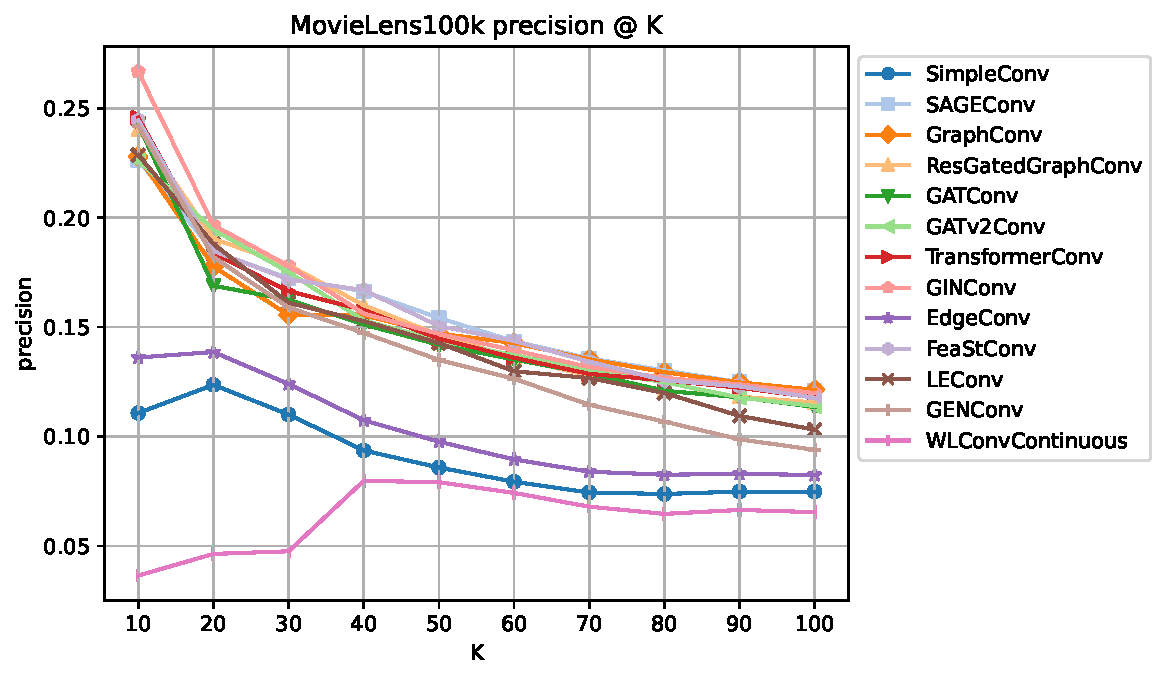
\includegraphics[width=\textwidth]{sn-article-template/imgs/MovieLens100k_precision.pdf}
    \captionof{figure}{MovieLens100k Results for Precision@$k$.}
    \label{fig:precision}
\end{minipage}

\begin{minipage}[b]{0.48\textwidth}
    \centering
    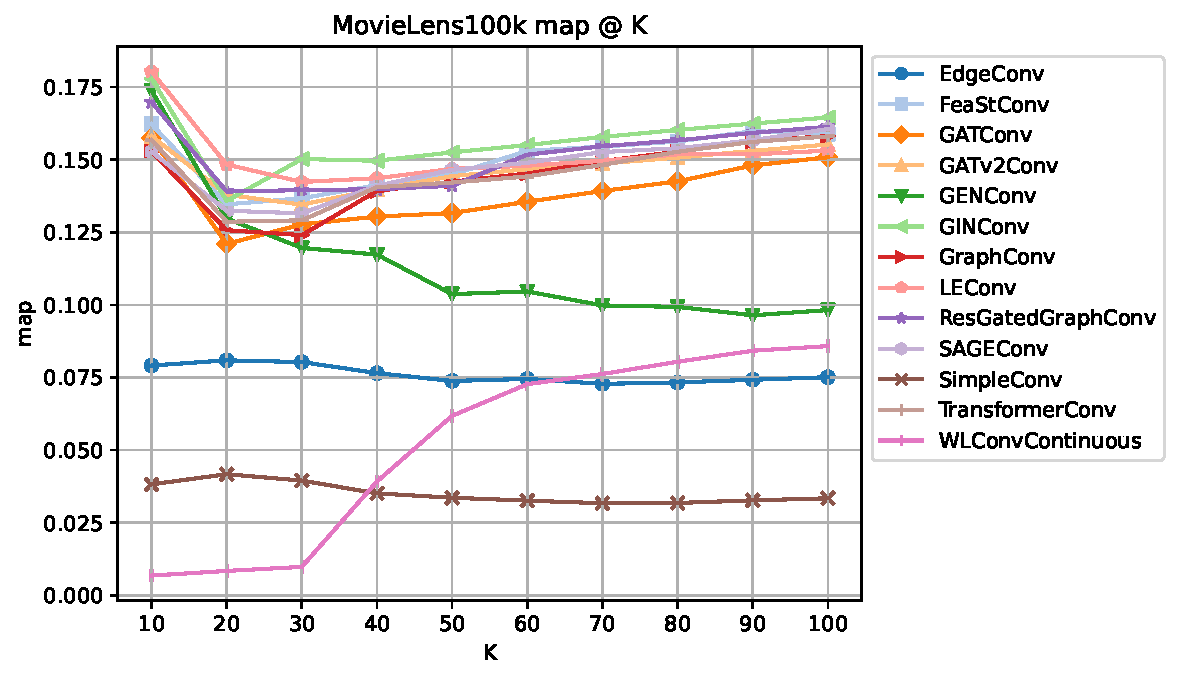
\includegraphics[width=\textwidth]{sn-article-template/imgs/MovieLens100k_map.pdf}
    \captionof{figure}{MovieLens100k Results for MAP@$k$.}
    \label{fig:map}
\end{minipage}
\hfill
\begin{minipage}[b]{0.48\textwidth}
    \centering
    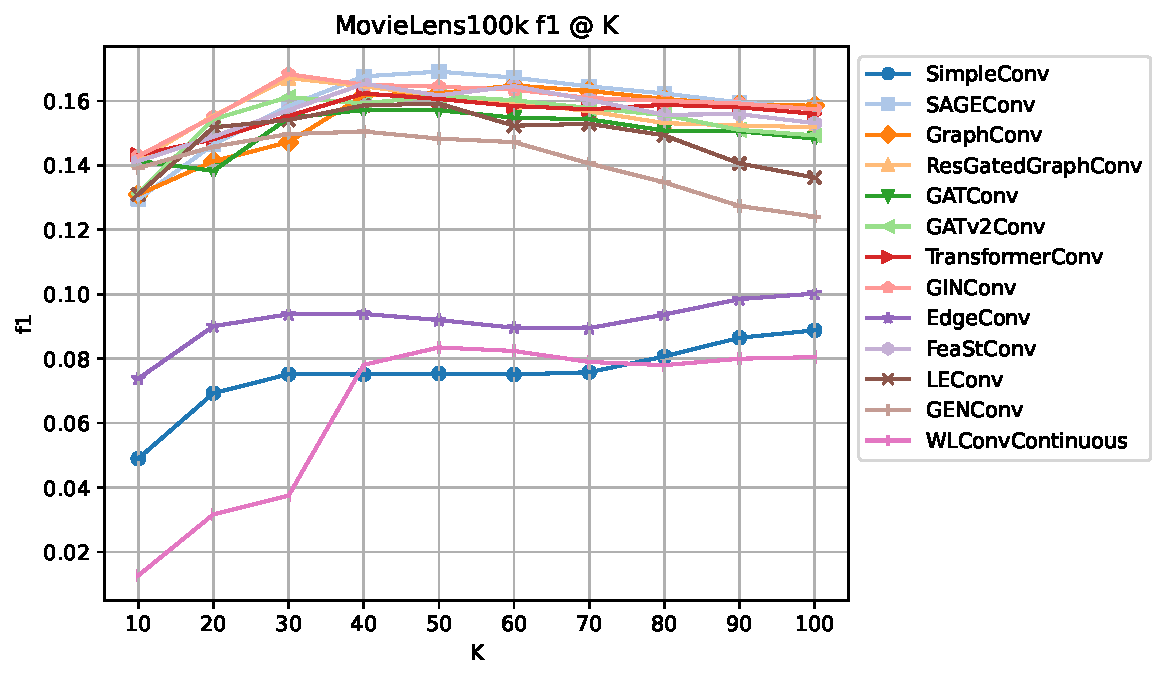
\includegraphics[width=\textwidth]{sn-article-template/imgs/MovieLens100k_f1.pdf}
    \captionof{figure}{MovieLens100k Results for F1@$k$.}
    \label{fig:f1}
\end{minipage}

\begin{minipage}[b]{0.48\textwidth}
    \centering
    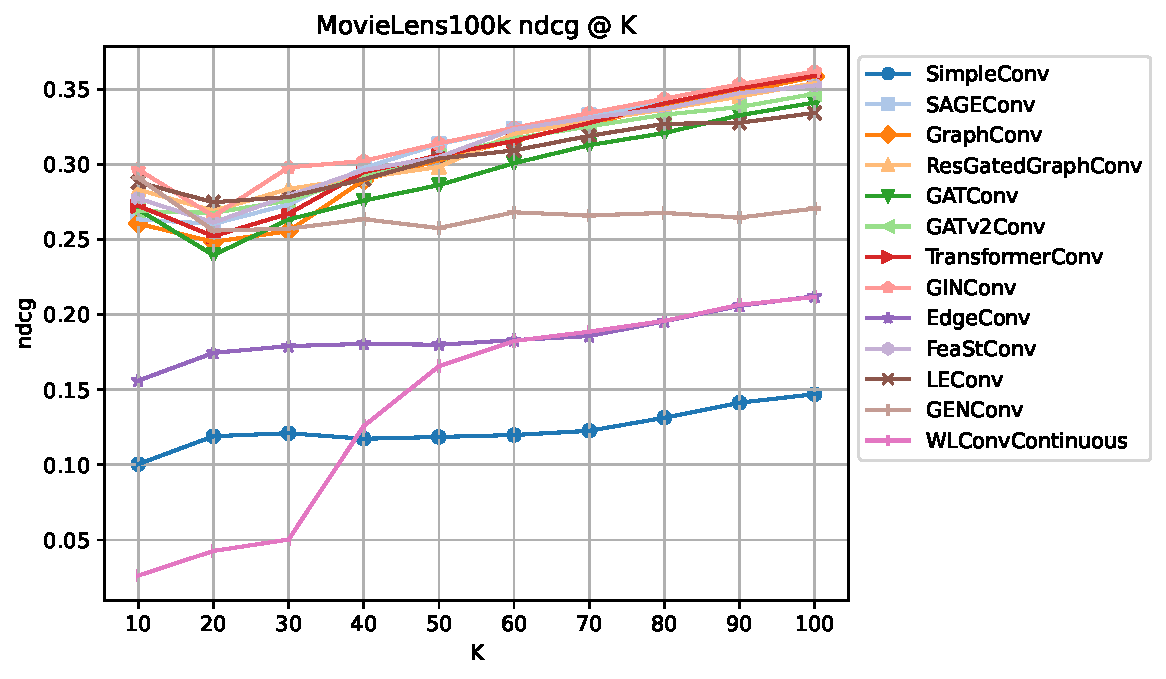
\includegraphics[width=\textwidth]{sn-article-template/imgs/MovieLens100k_ndcg.pdf}
    \captionof{figure}{MovieLens100k Results for nDCG@$k$.}
    \label{fig:ndcg}
\end{minipage}
\end{center}
\end{figure*}

\quad Both the figures and appendix tables \ref{secA3} present a comprehensive overview of the performance metrics of each bipartite GNN model applied to MovieLens100k dataset across different evaluation metrics, namely Recall@$k$, Precision@$k$, MAP@$k$, F1@$k$, and nDCG@$k$. Each figure and table focuses on a specific metric, providing results for different values of $k$, representing the top-$k$ recommendations. Overall, by first glance of the figures, the majority of the bipartite GNN models seem to have performed relatively the same, however there are three clear models that seem to have underperformed, these are: SimpleConv, WLConvContinuous and EdgeConv. The performance of the first two of the previously mentioned models was to be expected since they are comprised of aggregating input embeddings. Nevertheless, the underperformance of EdgeConv was not expected since the convolutional operator leverages neural networks.

In figure \ref{fig:recall} and table \ref{tab:recall}, the results for Recall@$k$ are displayed. Notably, the best performing models were SageConv, ResGatedGraphConv, TransformerConv and GINConv. However, from previously mentioned models TransformerConv had the most success when it came to achieving top scores for Recall@$k$, demonstrating its ability to dynamically recommend top-$k$ items from a list relevant items greater than 70.

In figure \ref{fig:precision} and table \ref{tab:precision}, the results for Precision@$k$ are displayed. Notably, the best performing models were SageConv, GraphConv, ResGatedGraphConv, GINConv and FeaStConv. However, from the previously mentioned models SAGEConv had the most success when it came to achieving top scores for Precision@$k$, demonstrating its ability to dynamically recommend top-$k$ items from a limited list relevant items roughly greater than 50.

In figure \ref{fig:map} and table \ref{tab:map}, the results for MAP@$k$ are displayed. Notably, GINConv and LEConv. However, from the previously mentioned models GINConv significantly stood over the rest when it came to achieving top scores for MAP@$k$, demonstrating its ability to dynamically rank relevant items across all users or queries.

In figure \ref{fig:f1} and table \ref{tab:f1}, the results for F1@$k$ are displayed. Notably, SageConv, GraphConv, ResGatedGraphConv, TransformerConv and GINConv. However, from the previously mentioned models SageConv significantly stood over the rest when it came to achieving top scores for F1@$k$, demonstrating a weighted ability to both dynamically provide and rank relevant items across all users or queries.

In figure \ref{fig:ndcg} and table \ref{tab:ndcg}, the results for nDCG@$k$ are displayed. Notably, GINConv and LEConv. However, from the previously mentioned models GINConv significantly stood over the rest when it came to achieving top scores for nDCG@$k$, demonstrating its ability to position dynamically relevant items across all users or queries.

Lastly, apart from the visually underperforming models mentioned at the beginning of this section, other models such as GATConv, GATv2Conv and GENConv were also unable to get a single top score for each metric at any given $k$.


% ------------------------------------------------------------------------------------------------------------------------

\section{Discussion}

\quad In table \ref{tab:aggregated}, an aggregation of the top-performing models across all metrics is presented. This table provides a summary of the most successful models based on their cumulative performance across the evaluated metrics. Noticeably, from the total column, we can observe that the two best models were GINConv with 22 top scores and SAGEConv with 11 top scores. This superior performance in our dynamic recommendation system benchmark can be attributed to their ability to effectively leverage graph structure, adaptively combine information from the target entity and its neighbors, and introduce flexibility and expressiveness through learnable parameters. These attributes enable GINConv and SAGEConv to capture intricate relationships and dependencies within the recommendation system, ultimately leading to improved recommendation performance.

For future work, we propose several avenues to further enhance dynamic recommendation systems. Firstly, exploring deeper architectures of Graph Neural Networks (GNNs) beyond GINConv and SAGEConv could unlock additional improvements in recommendation accuracy and personalization. Secondly, integrating Bipartite LSTMs into the recommendation framework offers a promising approach to modeling sequential interactions in bipartite graphs, potentially capturing temporal dynamics and long-term user preferences more effectively. Additionally, expanding the scope of datasets used for benchmarking could provide a more comprehensive evaluation of recommendation algorithms across diverse domains and scenarios. Lastly, leveraging more advanced computing resources such as AWS EC2 instances could facilitate extensive experimentation and model training, enabling us to tackle larger-scale recommendation problems and explore more complex architectures effectively.



% ------------------------------------------------------------------------------------------------------------------------
\section{Conclusion}

\quad In this research, we embarked on a meticulous exploration of Graph Neural Networks (GNNs) applied to dynamic recommendation systems within the context of undirected bipartite graphs. Our primary objective was to establish a standardized benchmarking framework to systematically evaluate the efficacy of various GNN operators tailored for this domain. To achieve this, we meticulously curated a comprehensive set of GNN models ranging from traditional techniques to state-of-the-art architectures, leveraging the PyTorch Geometric library for implementation.

Our contributions were threefold. Firstly, we developed a flexible and extensible benchmarking framework that encompasses data preprocessing, model training, evaluation protocols, and result analysis. This framework enables fair comparison and evaluation of GNN-based recommendation models under different experimental settings. Secondly, we rigorously evaluated the performance of each GNN operator on the MovieLens100k dataset, shedding light on their strengths and weaknesses in capturing intricate user-item interactions. Lastly, through insightful analysis of experimental results, we provided practical recommendations for selecting and configuring GNN models tailored to specific application domains, aiming to empower researchers and practitioners in the field.

By offering this comprehensive benchmarking study along with an open-source implementation in PyTorch Geometric, we aim to foster transparency, reproducibility, and innovation in the development of GNN-based dynamic recommendation systems. We believe that our work serves as a valuable resource for the community, facilitating advancements in recommendation engine technology and ultimately enhancing user experiences across various domains.

\begin{appendices}

\clearpage

\section{Summary of Models}\label{secA1}

\begin{longtable}{|l|l|l|}
    \hline
    \textbf{Model} & \textbf{Equations} \\
    \hline
    \endfirsthead
    
    \hline
    \textbf{Model} & \textbf{Equations} \\
    \hline
    \endhead
    
    \endfoot
    
    \hline
    \rowcolor[gray]{0.9} & \\
    \rowcolor[gray]{0.9} SimpleConv & $\mathbf{x}^{\prime}_{item_{i}} = \bigoplus_{j \in \mathcal{N}(i)} \mathbf{x}_{item_{j}}$ \\
    \rowcolor[gray]{0.9} & \\
    \rowcolor[gray]{0.9} & $\mathbf{x}^{\prime}_{user_{i}} = \bigoplus_{j \in \mathcal{N}(i)} \mathbf{x}_{user_{j}}$ \\
    \rowcolor[gray]{0.9} & \\

     & \\
    SAGEConv & $\mathbf{x}^{\prime}_{item_{i}} = \mathbf{W}_1 \mathbf{x}_{item_{i}} + \mathbf{W}_2 \cdot \mathrm{mean}_{j \in \mathcal{N}(i)} \mathbf{x}_{item_{j}}$ \\
     & \\
    & $\mathbf{x}^{\prime}_{user_{i}} = \mathbf{W}_1 \mathbf{x}_{user_{i}} + \mathbf{W}_2 \cdot \mathrm{mean}_{j \in \mathcal{N}(i)} \mathbf{x}_{user_{j}}$ \\
     & \\
    
    \rowcolor[gray]{0.9} & \\
    \rowcolor[gray]{0.9} GraphConv & $\mathbf{x}^{\prime}_{item_{i}} = \mathbf{W}_1 \mathbf{x}_{item_{i}} + \mathbf{W}_2 \cdot \sum_{j \in \mathcal{N}(i)} \mathbf{x}_{item_{j}}$ \\
    \rowcolor[gray]{0.9} & \\
    \rowcolor[gray]{0.9} & $\mathbf{x}^{\prime}_{user_{i}} = \mathbf{W}_1 \mathbf{x}_{user_{i}} + \mathbf{W}_2 \cdot \sum_{j \in \mathcal{N}(i)} \mathbf{x}_{user_{j}}$ \\
    \rowcolor[gray]{0.9} & \\

     & \\
    ResGatedGraphConv & $\mathbf{x}^{\prime}_{item_{i}} = \mathbf{W}_1 \mathbf{x}_{item_{i}} + \sum_{j \in \mathcal{N}(i)} \eta_{i,j} \odot \mathbf{W}_2 \mathbf{x}_{item_{j}}$\\
    & $\eta_{i,j} = \sigma(\mathbf{W}_3 \mathbf{x}_{item_{i}} + \mathbf{W}_4 \mathbf{x}_{item_{j}})$  \\
     & \\
    & $\mathbf{x}^{\prime}_{user_{i}} = \mathbf{W}_1 \mathbf{x}_{user_{i}} + \sum_{j \in \mathcal{N}(i)} \eta_{i,j} \odot \mathbf{W}_2 \mathbf{x}_{user_{j}}$\\
    & $\eta_{i,j} = \sigma(\mathbf{W}_3 \mathbf{x}_{user_{i}} + \mathbf{W}_4 \mathbf{x}_{user_{j}})$ \\
     & \\
    
    \rowcolor[gray]{0.9} & \\
    \rowcolor[gray]{0.9} GATConv & $\mathbf{x}^{\prime}_{item_{i}} = \alpha_{i,i}\mathbf{W}_{1}\mathbf{x}_{item_{i}} + \sum_{j \in \mathcal{N}(i)} \alpha_{i,j}\mathbf{W}_{2}\mathbf{x}_{item_{j}}$ \\
    \rowcolor[gray]{0.9} & $\alpha_{i,j} = \frac{\exp\left(\mathrm{LeakyReLU}\left(\mathbf{a}^{\top}_{1} \mathbf{W}_{1}\mathbf{x}_{item_{i}} + \mathbf{a}^{\top}_{2} \mathbf{W}_{2}\mathbf{x}_{item_{j}}\right)\right)}{\sum_{k \in \mathcal{N}(i) \cup \{ i \}}\exp\left(\mathrm{LeakyReLU}\left(\mathbf{a}^{\top}_{1} \mathbf{W}_{1}\mathbf{x}_{item_{i}} + \mathbf{a}^{\top}_{2}\mathbf{W}_{2}\mathbf{x}_{item_{k}}\right)\right)}$ \\
    \rowcolor[gray]{0.9} & \\
    \rowcolor[gray]{0.9} & $\mathbf{x}^{\prime}_{user_{i}} = \alpha_{i,i}\mathbf{W}_{1}\mathbf{x}_{user_{i}} + \sum_{j \in \mathcal{N}(i)} \alpha_{i,j}\mathbf{W}_{2}\mathbf{x}_{user_{j}}$ \\
    \rowcolor[gray]{0.9} & $\alpha_{i,j} = \frac{\exp\left(\mathrm{LeakyReLU}\left(\mathbf{a}^{\top}_{1} \mathbf{W}_{1}\mathbf{x}_{user_{i}} + \mathbf{a}^{\top}_{2} \mathbf{W}_{2}\mathbf{x}_{user_{j}}\right)\right)}{\sum_{k \in \mathcal{N}(i) \cup \{ i \}}\exp\left(\mathrm{LeakyReLU}\left(\mathbf{a}^{\top}_{1} \mathbf{W}_{1}\mathbf{x}_{user_{i}} + \mathbf{a}^{\top}_{2}\mathbf{W}_{2}\mathbf{x}_{user_{k}}\right)\right)}$ \\
    \rowcolor[gray]{0.9} & \\

     & \\
    GATv2Conv & $\mathbf{x}^{\prime}_{item_{i}} = \alpha_{i,i}\mathbf{W}_{1}\mathbf{x}_{item_{i}} + \sum_{j \in \mathcal{N}(i)} \alpha_{i,j}\mathbf{W}_{2}\mathbf{x}_{item_{j}}$\\
    & $\alpha_{i,j} = \frac{\exp\left(\mathbf{a}^{\top}\mathrm{LeakyReLU}\left(\mathbf{W}_{1} \mathbf{x}_{item_{i}} + \mathbf{W}_{2} \mathbf{x}_{item_{j}}\right)\right)}{\sum_{k \in \mathcal{N}(i) \cup \{ i \}} \exp\left(\mathbf{a}^{\top}\mathrm{LeakyReLU}\left(\mathbf{W}_{1} \mathbf{x}_{item_{i}} + \mathbf{W}_{2} \mathbf{x}_{item_{k}}\right)\right)}$ \\
     & \\
    & $\mathbf{x}^{\prime}_{user_{i}} = \alpha_{i,i}\mathbf{W}_{1}\mathbf{x}_{user_{i}} + \sum_{j \in \mathcal{N}(i)} \alpha_{i,j}\mathbf{W}_{2}\mathbf{x}_{user_{j}}$\\
    & $\alpha_{i,j} = \frac{\exp\left(\mathbf{a}^{\top}\mathrm{LeakyReLU}\left(\mathbf{W}_{1} \mathbf{x}_{user_{i}} + \mathbf{W}_{2} \mathbf{x}_{user_{j}}\right)\right)}{\sum_{k \in \mathcal{N}(i) \cup \{ i \}} \exp\left(\mathbf{a}^{\top}\mathrm{LeakyReLU}\left(\mathbf{W}_{1} \mathbf{x}_{user_{i}} + \mathbf{W}_{2} \mathbf{x}_{user_{k}}\right)\right)}$ \\
     & \\
    
    \rowcolor[gray]{0.9} & \\
    \rowcolor[gray]{0.9} TransformerConv & $\mathbf{x}^{\prime}_{item_{i}} = \mathbf{W}_1 \mathbf{x}_{item_{i}} + \sum_{j \in \mathcal{N}(i)} \alpha_{i,j} \mathbf{W}_2 \mathbf{x}_{item_{j}}$  \\
    \rowcolor[gray]{0.9} & $\alpha_{i,j} = \textrm{softmax} \left( \frac{(\mathbf{W}_3\mathbf{x}_{item_{i}})^{\top} (\mathbf{W}_4\mathbf{x}_{item_{j}})} {\sqrt{d}} \right)$ \\
    \rowcolor[gray]{0.9} & \\
    \rowcolor[gray]{0.9} & $\mathbf{x}^{\prime}_{user_{i}} = \mathbf{W}_1 \mathbf{x}_{user_{i}} + \sum_{j \in \mathcal{N}(i)} \alpha_{i,j} \mathbf{W}_2 \mathbf{x}_{user_{j}}$ \\
    \rowcolor[gray]{0.9} & $\alpha_{i,j} = \textrm{softmax} \left( \frac{(\mathbf{W}_3\mathbf{x}_{user_{i}})^{\top} (\mathbf{W}_4\mathbf{x}_{user_{j}})} {\sqrt{d}} \right)$ \\
    \rowcolor[gray]{0.9} & \\
    
     & \\
    GINConv & $\mathbf{x}^{\prime}_{item_{i}} = NN_{\mathbf{\Theta}} \left( (1 + \epsilon) \cdot \mathbf{x}_{item_{i}} + \sum_{j \in \mathcal{N}(i)} \mathbf{x}_{item_{j}} \right)$ \\
     & \\
    & $\mathbf{x}^{\prime}_{user_{i}} = NN_{\mathbf{\Theta}} \left( (1 + \epsilon) \cdot \mathbf{x}_{user_{i}} + \sum_{j \in \mathcal{N}(i)} \mathbf{x}_{user_{j}} \right)$ \\
     & \\
     
    \rowcolor[gray]{0.9} & \\
    \rowcolor[gray]{0.9} EdgeConv & $\mathbf{x}^{\prime}_{item_{i}} = \sum_{j \in \mathcal{N}(i)} NN_{\mathbf{\Theta}}(\mathbf{x}_{item_{i}} \, \Vert \, \mathbf{x}_{item_{j}} - \mathbf{x}_{item_{i}})$ \\
    \rowcolor[gray]{0.9} & \\
    \rowcolor[gray]{0.9} & $\mathbf{x}^{\prime}_{user_{i}} = \sum_{j \in \mathcal{N}(i)} NN_{\mathbf{\Theta}}(\mathbf{x}_{user_{i}} \, \Vert \, \mathbf{x}_{user_{j}} - \mathbf{x}_{user_{i}})$ \\
    \rowcolor[gray]{0.9} & \\

     & \\
    FeaStConv & $\mathbf{x}^{\prime}_{item_{i}} = \frac{1}{|\mathcal{N}(i)|} \sum_{j \in \mathcal{N}(i)} \sum_{h=1}^H
    q_h(\mathbf{x}_{item_{i}}, \mathbf{x}_{item_{j}}) \mathbf{W}_h \mathbf{x}_{item_{j}}$ \\
    & $q_h(\mathbf{x}_{item_{i}}, \mathbf{x}_{item_{j}}) = \mathrm{softmax}_{j}
    (\mathbf{u}_h^{\top} (\mathbf{x}_{item_{j}} - \mathbf{x}_{item_{i}}) + c_h)$ \\
     & \\
    &  $\mathbf{x}^{\prime}_{user_{i}} = \frac{1}{|\mathcal{N}(i)|} \sum_{j \in \mathcal{N}(i)} \sum_{h=1}^H
    q_h(\mathbf{x}_{user_{i}}, \mathbf{x}_{user_{j}}) \mathbf{W}_h \mathbf{x}_{user_{j}}$ \\
    & $q_h(\mathbf{x}_{user_{i}}, \mathbf{x}_{user_{j}}) = \mathrm{softmax}_j
    (\mathbf{u}_h^{\top} (\mathbf{x}_{user_{j}} - \mathbf{x}_{user_{i}}) + c_h)$ \\
     & \\

    \rowcolor[gray]{0.9} & \\
    \rowcolor[gray]{0.9} LEConv & $\mathbf{x}^{\prime}_{item_{i}} =  \mathbf{W}_1 \mathbf{x}_{item_{i}}+
    \sum_{j \in \mathcal{N}(i)}
    (\mathbf{W}_2 \mathbf{x}_{item_{i}} - \mathbf{W}_3 \mathbf{x}_{item_{j}})$ \\
    \rowcolor[gray]{0.9} & \\
    \rowcolor[gray]{0.9} & $\mathbf{x}^{\prime}_{user_{i}} = \mathbf{W}_1 \mathbf{x}_{user_{i}}+
    \sum_{j \in \mathcal{N}(i)}
    (\mathbf{W}_2 \mathbf{x}_{user_{i}} - \mathbf{W}_3 \mathbf{x}_{user_{j}})$ \\
    \rowcolor[gray]{0.9} & \\

     & \\
    GENConv & $\mathbf{x}_{item_{i}}^{\prime} = \mathrm{MLP} \left( \mathbf{x}_{item_{i}} +
    \sum_{j \in \mathcal{N}(i)} 
    \mathrm{ReLU} \left( \mathbf{x}_{item_{j}} \right) +\epsilon \right)$ \\
     & \\
     & $\mathbf{x}_{user_{i}}^{\prime} = \mathrm{MLP} \left( \mathbf{x}_{user_{i}} +
    \sum_{j \in \mathcal{N}(i)} 
    \mathrm{ReLU} \left( \mathbf{x}_{user_{j}} \right) +\epsilon \right)$ \\
     & \\

    \rowcolor[gray]{0.9} & \\
    \rowcolor[gray]{0.9} WLConvContinuous &     $\mathbf{x}^{\prime}_{item_{i}} = \frac{1}{2}\big(\mathbf{x}_{item_{i}} +
    \frac{1}{\textrm{deg}(i)}
    \sum_{j \in \mathcal{N}(i)}  \mathbf{x}_{item_{j}} \big)$ \\
    \rowcolor[gray]{0.9} & \\
    \rowcolor[gray]{0.9} & $\mathbf{x}^{\prime}_{user_{i}} = \frac{1}{2}\big(\mathbf{x}_{user_{i}} +
    \frac{1}{\textrm{deg}(i)}
    \sum_{j \in \mathcal{N}(i)} \mathbf{x}_{user_{j}} \big)$ \\
    \rowcolor[gray]{0.9} & \\
    
    \hline
    \caption{Summary of Bipartite GNN Models.}
    \label{tab:recall}
\end{longtable}

\clearpage

\section{Summary of Hyperparameters}\label{secA2}
 
\begin{table}[htbp]
    \centering
    \begin{tabular}{|l|c|c|c|c|} % Adjusted column widths
    \hline
    \textbf{Model} & \textbf{Bipartite GNN Layers} & \textbf{Linear Layers} & \textbf{Neural Networks} & \textbf{Heads} \\ % Adjusted headers
    \hline
    \rowcolor[gray]{0.9} SimpleConv & 1 & 1 & - & - \\
    SAGEConv & 2 & 2 & - & - \\
    \rowcolor[gray]{0.9} GraphConv & 2 & 2 & - & - \\
    ResGatedGraphConv & 2 & 2 & - & - \\
    \rowcolor[gray]{0.9} GATConv & 3 & 3 & - & 8 \\
    GATv2Conv & 3 & 3 & - & 8 \\
    \rowcolor[gray]{0.9} TransformerConv & 3 & - & - & 8 \\
    GINConv & 1 & 1 & 1MLP-3L & - \\
    \rowcolor[gray]{0.9} EdgeConv & 1 & 1 & 1MLP-2L & - \\
    FeaStConv & 2 & 3 & - & 2 \\
    \rowcolor[gray]{0.9} LEConv & 3 & 3 & - & - \\
    GENConv & 3 & 3 & - & - \\
    \rowcolor[gray]{0.9} WLConvContinuous & 3 & 3 & - & - \\
    \hline
    \end{tabular}
    \caption{Summary of Bipartite GNN Model Hyperparameters.}
    \label{tab:hyperparameters}
\end{table}

\clearpage

\section{Summary of Results}\label{secA3}

\vspace{1cm}

\begin{table}[htbp]
    \hspace{-2.3cm}
    \begin{tabular}{|l|*{10}{c|}}
    \hline
    \multirow{2}{*}{Model} & \multicolumn{10}{c|}{K} \\
    \hhline{~*{10}{|-}|}
                             & 10    & 20    & 30    & 40    & 50    & 60    & 70    & 80    & 90    & 100   \\ \hline
    \rowcolor[gray]{0.9} SimpleConv               & 0.0467 & 0.0731 & 0.0990 & 0.1120 & 0.1281 & 0.1404 & 0.1551 & 0.1816 & 0.2081 & 0.2205 \\ 
    SAGEConv                 & 0.1346 & 0.1965 & 0.2471 & 0.2989 & \textbf{0.3426} & 0.3771 & 0.4004 & 0.4223 & 0.4437 & 0.4608 \\ 
    \rowcolor[gray]{0.9} GraphConv                & 0.1364 & 0.1907 & 0.2355 & 0.2955 & 0.3298 & 0.3628 & 0.3932 & 0.4274 & 0.4494 & 0.4752 \\ 
    ResGatedGraphConv        & \textbf{0.1498} & \textbf{0.2136} & 0.2701 & 0.3040 & 0.3330 & \textbf{0.3780} & 0.4018 & 0.4228 & 0.4409 & 0.4589 \\ 
    \rowcolor[gray]{0.9} GATConv                  & 0.1461 & 0.1853 & 0.2488 & 0.2876 & 0.3197 & 0.3482 & 0.3729 & 0.3919 & 0.4118 & 0.4333 \\ 
    GATv2Conv                & 0.1381 & 0.2045 & 0.2518 & 0.2987 & 0.3396 & 0.3682 & 0.3890 & 0.4104 & 0.4268 & 0.4444 \\ 
    \rowcolor[gray]{0.9} TransformerConv          & 0.1485 & 0.2003 & 0.2535 & 0.3083 & 0.3412 & 0.3678 & \textbf{0.4060} & \textbf{0.4372} & \textbf{0.4603} & \textbf{0.4814} \\ 
    GINConv                  & 0.1458 & 0.2062 & \textbf{0.2740} & \textbf{0.3088} & 0.3419 & 0.3729 & 0.4014 & 0.4264 & 0.4475 & 0.4728 \\ 
    \rowcolor[gray]{0.9} EdgeConv                 & 0.0917 & 0.1311 & 0.1572 & 0.1835 & 0.1972 & 0.2132 & 0.2305 & 0.2631 & 0.2896 & 0.3039 \\ 
    FeaStConv                & 0.1458 & 0.2007 & 0.2446 & 0.2878 & 0.3194 & 0.3639 & 0.3885 & 0.4065 & 0.4327 & 0.4504 \\ 
    \rowcolor[gray]{0.9} LEConv                   & 0.1350 & 0.2004 & 0.2441 & 0.2840 & 0.3292 & 0.3475 & 0.3749 & 0.3935 & 0.4082 & 0.4237 \\ 
    GENConv                  & 0.1457 & 0.2028 & 0.2473 & 0.2822 & 0.3180 & 0.3602 & 0.3771 & 0.3857 & 0.3930 & 0.4066 \\ 
    \rowcolor[gray]{0.9} WLConvContinuous         & 0.0174 & 0.0396 & 0.0536 & 0.1380 & 0.1697 & 0.1836 & 0.1943 & 0.2062 & 0.2178 & 0.2288 \\ \hline
    \end{tabular}
    \caption{MovieLens100k Results for Recall@$k$.}
    \label{tab:recall}
\end{table}

\begin{table}[htbp]
    \hspace{-2.3cm} 
    \begin{tabular}{|l|*{10}{c|}}
    \hline
    \multirow{2}{*}{Model} & \multicolumn{10}{c|}{K} \\
    \hhline{~*{10}{|-}|}
                             & 10    & 20    & 30    & 40    & 50    & 60    & 70    & 80    & 90    & 100   \\ \hline
    \rowcolor[gray]{0.9} SimpleConv               & 0.1107 & 0.1236 & 0.1100 & 0.0936 & 0.0858 & 0.0793 & 0.0744 & 0.0737 & 0.0748 & 0.0748 \\ 
    SAGEConv                 & 0.2264 & 0.1846 & 0.1723 & 0.1663 & \textbf{0.1542} & 0.1435 & \textbf{0.1357} & \textbf{0.1302} & \textbf{0.1248} & 0.1210 \\ 
    \rowcolor[gray]{0.9} GraphConv                & 0.2279 & 0.1777 & 0.1555 & 0.1554 & 0.1470 & 0.1427 & 0.1353 & 0.1294 & 0.1247 & \textbf{0.1213} \\ 
    ResGatedGraphConv        & 0.2404 & 0.1904 & \textbf{0.1783} & 0.1600 & 0.1464 & 0.1359 & 0.1278 & 0.1208 & 0.1182 & 0.1155 \\ 
    \rowcolor[gray]{0.9} GATConv                  & 0.2425 & 0.1689 & 0.1625 & 0.1512 & 0.1419 & 0.1352 & 0.1288 & 0.1209 & 0.1179 & 0.1135 \\ 
    GATv2Conv                & 0.2261 & 0.1946 & 0.1751 & 0.1530 & 0.1439 & 0.1371 & 0.1303 & 0.1248 & 0.1178 & 0.1139 \\ 
    \rowcolor[gray]{0.9} TransformerConv          & 0.2457 & 0.1838 & 0.1664 & 0.1578 & 0.1447 & 0.1360 & 0.1286 & 0.1257 & 0.1223 & 0.1178 \\ 
    GINConv                  & \textbf{0.2668} & \textbf{0.1966} & 0.1780 & 0.1562 & 0.1469 & 0.1394 & 0.1317 & 0.1268 & 0.1238 & 0.1198 \\ 
    \rowcolor[gray]{0.9} EdgeConv                 & 0.1361 & 0.1386 & 0.1240 & 0.1074 & 0.0976 & 0.0895 & 0.0839 & 0.0825 & 0.0829 & 0.0824 \\ 
    FeaStConv                & 0.2446 & 0.1848 & 0.1718 & \textbf{0.1669} & 0.1505 & \textbf{0.1437} & 0.1342 & 0.1257 & 0.1229 & 0.1177 \\ 
    \rowcolor[gray]{0.9} LEConv                   & 0.2286 & 0.1880 & 0.1611 & 0.1527 & 0.1427 & 0.1298 & 0.1267 & 0.1199 & 0.1094 & 0.1031 \\ 
    GENConv                  & 0.2421 & 0.1820 & 0.1590 & 0.1473 & 0.1350 & 0.1264 & 0.1145 & 0.1068 & 0.0987 & 0.0939 \\ 
    \rowcolor[gray]{0.9} WLConvContinuous         & 0.0364 & 0.0463 & 0.0475 & 0.0797 & 0.0791 & 0.0742 & 0.0679 & 0.0646 & 0.0664 & 0.0654 \\ \hline
    \end{tabular}
    \caption{MovieLens100k Results for Precision@$k$.}
    \label{tab:precision}
\end{table}

\begin{table}[htbp]
    \hspace{-2.3cm}
    \begin{tabular}{|l|*{10}{c|}}
    \hline
    \multirow{2}{*}{Model} & \multicolumn{10}{c|}{K} \\
    \hhline{~*{10}{|-}|}
                             & 10    & 20    & 30    & 40    & 50    & 60    & 70    & 80    & 90    & 100   \\ \hline
    \rowcolor[gray]{0.9} SimpleConv               & 0.0382 & 0.0417 & 0.0395 & 0.0351 & 0.0336 & 0.0326 & 0.0317 & 0.0318 & 0.0327 & 0.0334 \\ 
    SAGEConv                 & 0.1527 & 0.1324 & 0.1315 & 0.1410 & 0.1465 & 0.1489 & 0.1526 & 0.1539 & 0.1567 & 0.1605 \\ 
    \rowcolor[gray]{0.9} GraphConv                & 0.1528 & 0.1257 & 0.1240 & 0.1392 & 0.1424 & 0.1452 & 0.1495 & 0.1527 & 0.1564 & 0.1581 \\ 
    ResGatedGraphConv        & 0.1698 & 0.1390 & 0.1395 & 0.1398 & 0.1410 & 0.1517 & 0.1546 & 0.1566 & 0.1592 & 0.1613 \\ 
    \rowcolor[gray]{0.9} GATConv                  & 0.1574 & 0.1210 & 0.1277 & 0.1304 & 0.1316 & 0.1355 & 0.1392 & 0.1425 & 0.1480 & 0.1508 \\ 
    GATv2Conv                & 0.1581 & 0.1379 & 0.1345 & 0.1397 & 0.1443 & 0.1467 & 0.1486 & 0.1507 & 0.1530 & 0.1552 \\ 
    \rowcolor[gray]{0.9} TransformerConv          & 0.1568 & 0.1286 & 0.1291 & 0.1405 & 0.1421 & 0.1442 & 0.1482 & 0.1527 & 0.1561 & 0.1580 \\ 
    GINConv                  & 0.1778 & 0.1358 & \textbf{0.1502} & \textbf{0.1496} & \textbf{0.1525} & \textbf{0.1550} & \textbf{0.1578} & \textbf{0.1602} & \textbf{0.1624} & \textbf{0.1645} \\ 
    \rowcolor[gray]{0.9} EdgeConv                 & 0.0791 & 0.0809 & 0.0803 & 0.0765 & 0.0738 & 0.0745 & 0.0728 & 0.0733 & 0.0742 & 0.0751 \\ 
    FeaStConv                & 0.1622 & 0.1346 & 0.1367 & 0.1412 & 0.1448 & 0.1530 & 0.1545 & 0.1562 & 0.1598 & 0.1589 \\ 
    \rowcolor[gray]{0.9} LEConv                   & \textbf{0.1803} & \textbf{0.1483} & 0.1423 & 0.1436 & 0.1468 & 0.1479 & 0.1496 & 0.1518 & 0.1518 & 0.1531 \\ 
    GENConv                  & 0.1738 & 0.1297 & 0.1196 & 0.1173 & 0.1037 & 0.1046 & 0.0998 & 0.0993 & 0.0964 & 0.0982 \\ 
    \rowcolor[gray]{0.9} WLConvContinuous         & 0.0068 & 0.0084 & 0.0098 & 0.0392 & 0.0618 & 0.0727 & 0.0762 & 0.0804 & 0.0842 & 0.0858 \\ \hline
    \end{tabular}
    \caption{MovieLens100k Results for MAP@$k$.}
    \label{tab:map}
\end{table}

\begin{table}[htbp]
    \hspace{-2.3cm}
    \begin{tabular}{|l|*{10}{c|}}
    \hline
    \multirow{2}{*}{Model} & \multicolumn{10}{c|}{K} \\
    \hhline{~*{10}{|-}|}
                             & 10    & 20    & 30    & 40    & 50    & 60    & 70    & 80    & 90    & 100   \\ \hline
    \rowcolor[gray]{0.9} SimpleConv               & 0.0490 & 0.0693 & 0.0752 & 0.0751 & 0.0754 & 0.0751 & 0.0758 & 0.0807 & 0.0865 & 0.0888 \\ 
    SAGEConv                 & 0.1295 & 0.1465 & 0.1584 & \textbf{0.1676} & \textbf{0.1691} & \textbf{0.1672} & \textbf{0.1645} & \textbf{0.1623} & \textbf{0.1595} & 0.1581 \\ 
    \rowcolor[gray]{0.9} GraphConv                & 0.1309 & 0.1413 & 0.1472 & 0.1617 & 0.1624 & 0.1648 & 0.1631 & 0.1606 & 0.1589 & \textbf{0.1585} \\ 
    ResGatedGraphConv        & 0.1416 & \textbf{0.1554} & 0.1671 & 0.1645 & 0.1617 & 0.1595 & 0.1568 & 0.1531 & 0.1524 & 0.1518 \\ 
    \rowcolor[gray]{0.9} GATConv                  & 0.1414 & 0.1383 & 0.1547 & 0.1572 & 0.1571 & 0.1548 & 0.1543 & 0.1508 & 0.1506 & 0.1483 \\ 
    GATv2Conv                & 0.1313 & 0.1543 & 0.1612 & 0.1592 & 0.1616 & 0.1602 & 0.1578 & 0.1556 & 0.1510 & 0.1493 \\ 
    \rowcolor[gray]{0.9} TransformerConv          & \textbf{0.1432} & 0.1481 & 0.1553 & 0.1623 & 0.1606 & 0.1584 & 0.1574 & 0.1588 & 0.1580 & 0.1560 \\ 
    GINConv                  & 0.1429 & 0.1550 & \textbf{0.1683} & 0.1650 & 0.1644 & 0.1635 & 0.1609 & 0.1600 & 0.1592 & 0.1574 \\ 
    \rowcolor[gray]{0.9} EdgeConv                 & 0.0738 & 0.0901 & 0.0938 & 0.0939 & 0.0920 & 0.0896 & 0.0895 & 0.0937 & 0.0985 & 0.1002 \\ 
    FeaStConv                & 0.1413 & 0.1489 & 0.1571 & 0.1653 & 0.1617 & 0.1646 & 0.1603 & 0.1557 & 0.1559 & 0.1531 \\ 
    \rowcolor[gray]{0.9} LEConv                   & 0.1310 & 0.1518 & 0.1541 & 0.1586 & 0.1592 & 0.1523 & 0.1529 & 0.1493 & 0.1406 & 0.1362 \\ 
    GENConv                  & 0.1392 & 0.1458 & 0.1497 & 0.1505 & 0.1483 & 0.1472 & 0.1406 & 0.1347 & 0.1274 & 0.1241 \\ 
    \rowcolor[gray]{0.9} WLConvContinuous         & 0.0127 & 0.0317 & 0.0375 & 0.0781 & 0.0835 & 0.0824 & 0.0790 & 0.0780 & 0.0800 & 0.0805 \\ \hline
    \end{tabular}
    \caption{MovieLens100k Results for F1@$k$.}
    \label{tab:f1}
\end{table}

\begin{table}[htbp]
    \hspace{-2.3cm}
    \begin{tabular}{|l|*{10}{c|}}
    \hline
    \multirow{2}{*}{Model} & \multicolumn{10}{c|}{K} \\
    \hhline{~*{10}{|-}|}
                             & 10    & 20    & 30    & 40    & 50    & 60    & 70    & 80    & 90    & 100   \\ \hline
    \rowcolor[gray]{0.9} SimpleConv               & 0.1004 & 0.1190 & 0.1210 & 0.1173 & 0.1185 & 0.1198 & 0.1226 & 0.1313 & 0.1413 & 0.1470 \\ 
    SAGEConv                 & 0.2634 & 0.2604 & 0.2733 & 0.2976 & 0.3135 & 0.3239 & 0.3328 & 0.3410 & 0.3489 & 0.3580 \\ 
    \rowcolor[gray]{0.9} GraphConv                & 0.2606 & 0.2484 & 0.2556 & 0.2896 & 0.3027 & 0.3165 & 0.3268 & 0.3392 & 0.3477 & 0.3585 \\ 
    ResGatedGraphConv        & 0.2832 & 0.2691 & 0.2837 & 0.2911 & 0.2983 & 0.3203 & 0.3291 & 0.3366 & 0.3452 & 0.3541 \\ 
    \rowcolor[gray]{0.9} GATConv                  & 0.2699 & 0.2396 & 0.2633 & 0.2759 & 0.2862 & 0.3008 & 0.3128 & 0.3209 & 0.3327 & 0.3412 \\ 
    GATv2Conv                & 0.2689 & 0.2677 & 0.2759 & 0.2922 & 0.3057 & 0.3172 & 0.3253 & 0.3331 & 0.3382 & 0.3470 \\ 
    \rowcolor[gray]{0.9} TransformerConv          & 0.2724 & 0.2522 & 0.2672 & 0.2948 & 0.3060 & 0.3156 & 0.3276 & 0.3406 & 0.3507 & 0.3589 \\ 
    GINConv                  & \textbf{0.2966} & 0.2656 & \textbf{0.2980} & \textbf{0.3023} & \textbf{0.3140} & \textbf{0.3243} & \textbf{0.3342} & \textbf{0.3437} & \textbf{0.3534} & \textbf{0.3618} \\ 
    \rowcolor[gray]{0.9} EdgeConv                 & 0.1560 & 0.1745 & 0.1790 & 0.1805 & 0.1799 & 0.1830 & 0.1857 & 0.1955 & 0.2058 & 0.2122 \\ 
    FeaStConv                & 0.2773 & 0.2613 & 0.2791 & 0.2962 & 0.3049 & 0.3234 & 0.3310 & 0.3371 & 0.3474 & 0.3526 \\ 
    \rowcolor[gray]{0.9} LEConv                   & 0.2881 & \textbf{0.2748} & 0.2783 & 0.2901 & 0.3039 & 0.3093 & 0.3190 & 0.3270 & 0.3277 & 0.3343 \\ 
    GENConv                  & 0.2910 & 0.2559 & 0.2572 & 0.2635 & 0.2576 & 0.2681 & 0.2660 & 0.2677 & 0.2646 & 0.2706 \\ 
    \rowcolor[gray]{0.9} WLConvContinuous         & 0.0262 & 0.0426 & 0.0502 & 0.1258 & 0.1656 & 0.1824 & 0.1886 & 0.1958 & 0.2065 & 0.2117 \\ \hline
    \end{tabular}
    \caption{MovieLens100k Results for nDCG@$k$.}
    \label{tab:ndcg}
\end{table}

\begin{table}[htbp]
    \centering 
    \begin{tabular}{|l|*{5}{c|}c|}
    \hline
    \multirow{2}{*}{Model} & \multicolumn{5}{c|}{Metrics} & \multirow{2}{*}{Total} \\
    \hhline{~*{5}{|-}|~|}
                             & Recall & Precision & MAP & F1 & nDCG & \\ \hline
    \rowcolor[gray]{0.9} SimpleConv               & - & - & - & - & - & - \\ 
    SAGEConv                 & 1 & 4 & - & 6 & - & 11 \\ 
    \rowcolor[gray]{0.9} GraphConv                & - & 1 & - & 1 & - & 2 \\ 
    ResGatedGraphConv        & 3 & 1 & - & 1 & - & 5 \\ 
    \rowcolor[gray]{0.9} GATConv                  & - & - & - & - & - & - \\ 
    GATv2Conv                & - & - & - & - & - & - \\ 
    \rowcolor[gray]{0.9} TransformerConv          & 4 & - & - & 1 & - & 5 \\ 
    GINConv                  & 2 & 2 & 8 & 1 & 9 & 22 \\ 
    \rowcolor[gray]{0.9} EdgeConv                 & - & - & - & - & - & - \\ 
    FeaStConv                & - & 2 & - & - & - & 2 \\ 
    \rowcolor[gray]{0.9} LEConv                   & - & - & 2 & - & 1 & 3 \\ 
    GENConv                  & - & - & - & - & - & - \\ 
    \rowcolor[gray]{0.9} WLConvContinuous         & - & - & - & - & - & - \\ \hline
    \end{tabular}
    \caption{MovieLens100k Aggregated Top Results.}
    \label{tab:aggregated}
\end{table}

\end{appendices}

\clearpage

\bibliographystyle{unsrt}
\bibliography{Report/sn-bibliography}


%------ To create Appendix with additional stuff -------%
%\newpage
%\appendix
%\section{Appendix}
%Put data files, CAD drawings, additional sketches, etc.

\end{document} 